\documentclass[letter,12pt]{book}
\usepackage[spanish]{babel}
\usepackage[bookmarks]{hyperref}

\usepackage[utf8x]{inputenc}
\usepackage{lmodern}
\usepackage{graphicx}
\usepackage{epstopdf}
\usepackage{pdflscape}
\usepackage{array}
\usepackage{hvfloat}
\usepackage{apacite} 
\usepackage{chngcntr} %para numeracion de figuras
\usepackage{mathtools}
\usepackage{supertabular}
\graphicspath{ {./imagenes/} }
\setcounter{secnumdepth}{3} % para que ponga 1.1.1.1 en subsubsecciones...
\setcounter{tocdepth}{3} % para que añada las subsubsecciones en el indice...


\let\tmp\oddsidemargin
\let\oddsidemargin\evensidemargin
\let\evensidemargin\tmp
\reversemarginpar

\makeatletter
\renewenvironment{thebibliography}[1]
     {\chapter*{\bibname}% <-- this line was changed from \chapter* to \section*
      \@mkboth{\MakeUppercase\bibname}{\MakeUppercase\bibname}%
      \list{\@biblabel{\@arabic\c@enumiv}}%
           {\settowidth\labelwidth{\@biblabel{#1}}%
            \leftmargin\labelwidth
            \advance\leftmargin\labelsep
            \@openbib@code
            \usecounter{enumiv}%
            \let\p@enumiv\@empty
            \renewcommand\theenumiv{\@arabic\c@enumiv}}%
      \sloppy
      \clubpenalty4000
      \@clubpenalty \clubpenalty
      \widowpenalty4000%
      \sfcode`\.\@m}
     {\def\@noitemerr
       {\@latex@warning{Empty `thebibliography' environment}}%
      \endlist}
\makeatother

\setlength{\parskip}{1ex}

\newcolumntype{L}[1]{>{\raggedright\let\newline\\\arraybackslash\hspace{0pt}}m{#1}}
\newcolumntype{C}[1]{>{\centering\let\newline\\\arraybackslash\hspace{0pt}}m{#1}}
\newcolumntype{R}[1]{>{\raggedleft\let\newline\\\arraybackslash\hspace{0pt}}m{#1}}

\begin{document}

  \begin{titlepage}

    \begin{center}
      \vspace*{-1in}
      \begin{figure}[htb]
    \begin{center}
      
\includegraphics[width=8cm]{imagenes/Logo_Distrital.eps}
    \end{center}
    \end{figure}

    FACULTAD DE INGENIERÍA\\
    \vspace*{0.15in}
    PROYECTO CURRICULAR DE INGENIERÍA DE SISTEMAS \\
    \vspace*{0.6in}
    \begin{large}
    Proyecto:\\
    \end{large}
    \vspace*{0.2in}
    \begin{Large}
    \textbf{DISEÑO E IMPLEMENTACIÓN DE UN PROTOTIPO DE SNS ORIENTADO AL DEPORTE SOBRE TECNOLOGÍAS MÓVILES} \\ 
    \end{Large}
    \vspace*{0.3in}
    \begin{large}
    Presentado por:\\
      Nicolás Mauricio Garcia Garzon 20091020031 \\
      Luis Felipe Gonzalez Moreno 20091020035
    \end{large}
    \vspace*{0.3in}
    \rule{80mm}{0.1mm}\\
    \vspace*{0.1in}
    \begin{large}
    Dirigida por: \\
    Doctor Carlos Enrique Montenegro Marin
    \end{large}
    \end{center}

    \end{titlepage}



  \newpage
  \mbox{}
  \thispagestyle{empty} % para que no se numere esta página
  
  \tableofcontents % indice de contenidos

  \cleardoublepage
  \addcontentsline{toc}{chapter}{Lista de figuras} % para que aparezca en el indice de contenidos
  \listoffigures % indice de figuras

  \cleardoublepage
  \addcontentsline{toc}{chapter}{Lista de tablas} % para que aparezca en el indice de contenidos
  \listoftables % indice de tablas
  
  \counterwithout{figure}{chapter}
  \counterwithout{table}{chapter}
  
  \chapter*{Introducción} % si no queremos que añada la palabra "Capitulo"
  \addcontentsline{toc}{section}{Introducción} % si queremos que aparezca en el índice
  \markboth{INTRODUCCIÓN}{INTRODUCCIÓN} % encabezado
  El uso de los medios informáticos para la formación de comunidades deportivas en las que los deportistas puedan formar y gestionar sus redes sociales es restringido debido al modo de vida del deportista. Es usual que por medio de facebook y twitter los deportistas creen sus redes sociales. Sin embargo, facebook y twitter añaden información basura para los deportistas y no ofrecen servicios que han de ser propios de una red social deportiva.

En este documento se expone una propuesta para el desarrollo de una red social deportiva por medio de la teoría de redes sociales y SOA, así como la investigación del estado del arte de las redes sociales deportivas. Lo que se pretende con el documento es exponer el problema existente que hay entre la utilización de las TIC y la comunicación (a modo de red social) entre las comunidades deportivas y, además, se pretende exponer el desarrollo de un prototipo de SNS que resuelva dicho problema.

Primero, el lector encontrará un acercamiento al problema que se resolverá en la definición del problema, la justificación y los objetivos. Más adelante, el lector podrá echar un vistazo a la teoría que está detrás del problema a resolver y que es necesaria para su solución. Se presenta también al lector el marco a utilizar para la solución del problema en las secciones de metodología, cronograma y un estudio de presupuestos. Por último, el documento contiene los análisis funcionales, la creación de la arquitectura y del modelo de datos que llevará el prototipo de SNS construido.

  
  \chapter*{Glosario}
  \addcontentsline{toc}{section}{Glosario} % si queremos que aparezca en el índice
  \markboth{GLOSARIO}{GLOSARIO} % encabezado
  \begin{itemize}
  \item OSN : Online Social Network – Red Social En-línea, es una red social que crece dentro del ámbito web.
  \item SNS : Social Network Services – Servicios de Redes Sociales.
  \item Offline Social Network : Red social que crece en el ámbito real, no en el virtual como lo es en las OSN.
  \item Sistemas transversales : Sistemas que interactúan entre sí, hechos o no con tecnologías diferentes sobre paradigmas diferentes, con un fin común.
  \item API : Application Programming Interface – Interfaz de programas de aplicación, es el conjunto de funciones y procedimientos de un sistema que pueden ser utilizados en otro sistema. Es el puente de conexión entre ambos sistemas.
  \item Interoperabilidad : Capacidad de un sistema de software para trabajar con otro sistema con la característica de que esta cooperación sea hecha de la manera más transparente posible.
  \item SOA : Service-Oriented Architecture – Arquitectura Orientada a Servicios.
  \item TI : Tecnologías de la Información
  \item ROI : Return on investment – Retorno en inversión.
  \item Product Backlog : Productos que están pendientes por realizar para finalizar el proyecto.
  \item Sprint Goal : El objetivo, que de cumplirse, determina si el Sprint fue exitoso.
  \item Nodo : Punto de intersección de varios elementos
  \item Arista : Uniones entre nodos
  \item StakeHolders : Partes interesadas en un tema específico.
\end{itemize}

  
  \chapter{Definición del problema}
  \label{chap:definicion_problema}
  El hombre, en su continua evolución, ha utilizado el lenguaje como una herramienta creadora de conocimiento transferible a sus congéneres o cualquier otro ser que interactuase con él. Con esto, “los humanos han desarrollado el lenguaje como un instrumento ligero y conveniente para mantener sus relaciones”\cite{dynamics}. 

En la comunicación entre congéneres, el lenguaje puede ser dividido en dos funciones: función de transmisión de información (gossip) y función de entendimiento del estado interno (estado mental) del congénere (mentalisation)\cite{dynamics}. Estas funciones de transmisión y entendimiento del otro han permitido que dos o varios humanos puedan asociarse entre sí formando redes sociales.

Las redes sociales no son otra cosa que la formación de lazos de algún tipo (emocional, de pertenencia a una comunidad, de trabajo, etc.) entre individuos que pueden ser organizaciones o humanos.\cite{sna_startups} En la figura \ref{fig:red_al_quaeda} puede verse cómo es representada la red social que forman las células terroristas de Al-Qaeda.

\begin{figure}[!htb]
  \begin{center}
    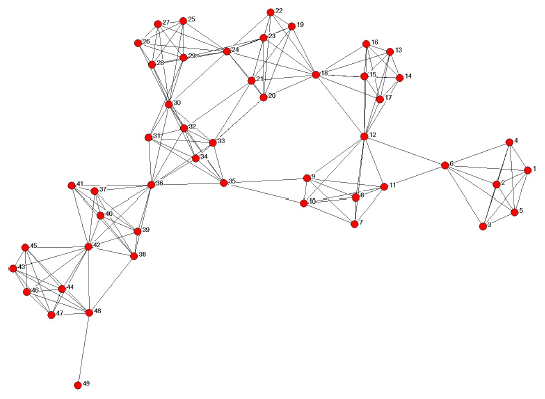
\includegraphics[width=11cm]{./imagenes/red_al_qaeda.png}
    \caption{Red social conformada por las células terroristas de Al-Qaeda.}
    \label{fig:red_al_quaeda}
  \end{center}
\end{figure}

La evolución de los servicios proporcionados a través de la internet ha sido drástica puesto que ha cambiado el modo de vida de las personas. En la figura \ref{fig:utilizacion_internet} se evidencia el crecimiento de la internet (de los servicios que en ella se soportan) se da en función de los servicios de conectividad social que son creados y soportados en ella. La web 1.0 fue utilizada en mayor medida por científicos para el intercambio de información en formato hipertexto. No había una interacción fuerte entre cada científico sino que ellos acudían a internet para buscar o poner a disposición material científico. Con la venida de la web 2.0 y la introducción de la interacción del usuario con la web generando contenido en tiempo real, así se crearon servicios de redes sociales en-línea (OSN en inglés: On-line Social Network), produciento una partición en los tipos de redes sociales. Así, las redes sociales a las que pertenece el ser humano en la era digital se dividieron convenientemente en “redes sociales fuera de línea” y redes sociales en línea (Offline Social Network y Online Social Network).

\begin{figure}[!htb]
  \begin{center}
    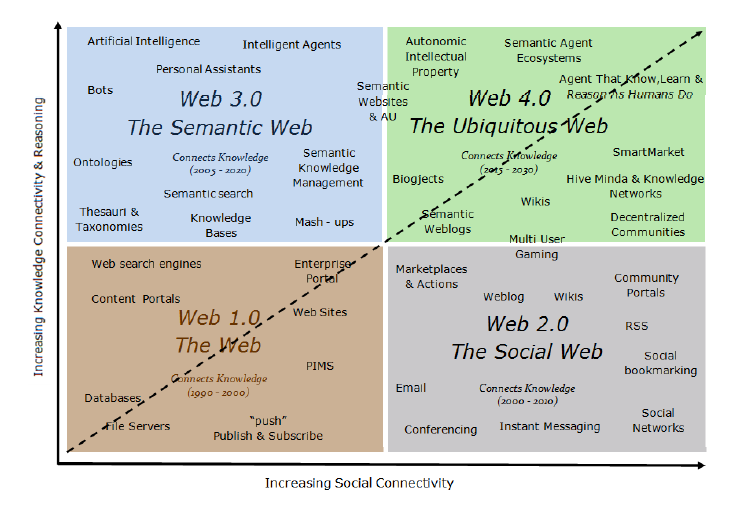
\includegraphics[width=11cm]{./imagenes/utilizacion_internet.png}
    \caption{Cambio de la utilización de internet en función de los servicios de conectividad social que son creados y soportados en ella}
    \label{fig:utilizacion_internet}
  \end{center}
\end{figure}

Las redes sociales fuera de línea son las redes sociales que se forman por comunicación tradicional (lenguaje oral y escrito en medios que difieran de aquellos que utilizan las telecomunicaciones). Las redes sociales en línea son aquellas redes sociales que están formadas por cibernautas y en las cuales la comunicación se da por medio de los servicios de redes sociales.

La administración de una red social fuera de línea fue estudiada desde inicios del siglo XX\cite{dynamics} con un enfoque socio-matemático llamado “análisis de redes sociales” (SNA por sus siglas en ingles: Social Network Analisis). Sin embargo, era difícil el análisis del comportamiento humano según los designios de la SNA puesto que la información debía ser recopilada por medio de entrevistas a las personas. Aún así, el enfoque SNA fue utilizado para analizar el comportamiento terrorista o inclusive el comportamiento de trabajadores en una empresa.\cite{sna_startups}

Con la creación de las OSN y la gran cantidad de información que describe el comportamiento humano sobre este tipo de red social, ha sido más sencillo utilizar el enfoque de la SNA para estudiar que comportamientos tienen los humanos sobre una red social establecida.

Los servicios de redes sociales (SNS por sus siglas en ingles: Social Network Services) como Facebook, LinkedIn, Twitter, SportTracker o Xportia, ofrecen servicios para la gestión de la OSN de cada usuario que acceda a estas aplicaciones. Según un estudio hecho para medir la experiencia de usuario (UX por sus siglas en ingles: User eXperience) en los SNS, se encontraron 8 categorías que son críticas a la hora de diseñar una SNS y son:

1. Self-expresion: Capacidad que tengan las OSN de compartir contenido relacionado a la vida real de los usuarios tal como lo pueden ser las fotos, los videos, los comentarios o las comunicaciones directas.
2. Reciprocity: Interacción bilateral en tiempo real, es decir, interacción instantánea con uno o varios individuales en la OSN (por ejemplo, por medio de los servicios de mensajería instantánea).
3. Learning: La información recibida por medio de la OSN debe poder ser utilizada en pro del desarrollo cognitivo del individual; debe existir información útil al individual que usa la OSN.
4. Curiosity: El contenido de la OSN debe ser interesante para quien la utiliza.
5. Suitability of functionality: Se refiere a cuán “utilizable” es una funcionalidad.
6. Suitability of content: La calidad y exactitud de la información que en la OSN reside debe ser suficiente para el individual perteneciente a ella.
7. Completeness of the user network: Los individuales deben querer pertenecer a la red social y buscar eficientemente a otros individuales para poder formar lazos con ellos y hacer crecer su red social.
8. Trust and privacy: Confianza en los servicios de las OSN, así como también la capacidad que tiene el usuario de gestionar la privacidad del contenido que comparte en dicha OSN.\cite{social_experience}

De acuerdo al enfoque SNA, las redes sociales pueden estar divididas en clusters, que no son más que agrupaciones de individuales sobre una red social por algún concepto como, por ejemplo, la pertenencia a una comunidad. Con lo anterior, podemos encontrar que algunos SNS ofrecen servicios para gestionar las OSN de sus usuarios centrándose en algún tipo de comunidad en específico y, la información que circula por ese tipo de comunidades, es diferente a la que pasa por SNS descentralizados (como Facebook y twitter). Viendo Facebook como una agrupación de clusters con temáticas tan diferentes como lo son los deportes y la música, la ciencia y la vida cotidiana, se puede decir que algunos SNS se enfocan en alguna de estas temáticas. En este caso, el cluster o temática que compete al trabajo a elaborar es el deporte.

Es posible hacer una división del cluster deporte en otros subclusters de cada uno de los deportes que existen en el mundo o en la clasificación de los deportes que han dado organizaciones como, por ejemplo, la IWGA (Internation WorldGames Association). Lo que se quiere con este trabajo es aportar al crecimiento de las redes sociales fuera de linea de las personas que practiquen deporte sin importar si lo hacen a nivel profesional o aficionado por medio de un SNS orientado a los deportes en general y, por lo tanto, el cluster que se ha escogido para trabajar es el del deporte como cluster mismo.

Se investigó acerca de las redes sociales existentes enfocadas a la temática del deporte y se encontró que muchas de ellas son utilizadas en mayor medida en España y que todas ellas están soportadas sobre tecnologías web. En general, solo se encontraron dos redes sociales deportivas orientadas a cualquier deporte asociadas a aplicaciones para smartphones disponibles en el la tienda virtual de Android o en la tienda virtual de Apple (La red social de Fitivity y Huddlers).

Así, con la evolución de la comunicación humana trasladándose a los espacios virtuales por medio de las OSN y la falta de aplicaciones, en el campo de los smartphones, que soporten interacciones sociales enfocadas a los deportes en general, en este trabajo se creará un SNS centrado en los deportes sobre tecnologías Android para la administración de las OSN de cada persona en un ámbito deportivo desde su dispositivo móvil.

  
  \chapter{Justificación del problema}
  Los humanos, desde siempre en su evolución, han necesitado de mecanismos para comunicarse con sus congéneres. En la actualidad, uno de los mecanismos es el uso de los SNS como facebook y twitter, cada uno de ellos modificando la forma de creación de redes sociales en la actualidad. (Sección \ref{sec:red})

De acuerdo al análisis egocéntrico de las redes sociales de cada individuo, se hace conveniente la utilización de SNS para gestionar las relaciones que un individuo mantiene con otros individuos (sean personas u organizaciones) en los diferentes círculos sociales en los que se mueve. (Sección \ref{sec:egocentrico})

El círculo social o comunidad escogida para el desarrollo propuesto es la comunidad deportiva debido a que hay mucha información dispersa alrededor de internet que es ambigua y a veces inclusive errónea. A su vez, debido a que gran cantidad de deportes no han tenido una acogida grande alrededor del mundo, las comunidades que se mueven sobre uno de esos deportes son más cerradas y, por ende, pequeñas y con poca información para un público que salga de las fronteras de dichas comunidades cerradas. Lo que se quiere con este trabajo es aportar al crecimiento de las redes sociales de las personas que practiquen deporte sin importar si lo hacen a nivel profesional o aficionado por medio de un SNS orientado a los deportes en general.

Un factor de utilización masiva de las SNS es que éstas estén orientadas a un público en particular y aumenten su cobertura dependiendo de su alcance de masa crítica sobre una red social definida \cite{sna_startups}. Al construir, en principio, la red social deportiva enfocada en dos deportes en particular, la probabilidad de ganar la masa crítica es mayor y, por tanto, el SNS desarrollado puede volverse más útil con el tiempo.

La UX de los SNS (visto en el capítulo \ref{cap:estado_arte}) es otro factor, debido a que juega un papel importante pues es esta la segunda carta de presentación de un SNS. Algunas de las características que evalúan los usuarios en cuanto a la UX no son suplidas por los SNS actuales – o al menos no parcialmente - , tres de ellas (fundamentales para la acogida de un nuevo SNS) son “curiosity, learning y completeness of the social network”. Así, habiendo analizado 19 SNS orientados al deporte (Tablas \ref{tab:comparacion_redes_1} a \ref{tab:comparacion_redes_5}), se concluyó que fallaban en alguna de las tres características mencionadas.

Tener en cuenta la población a quien va dirigido el SNS a desarrollar es otro factor de éxito. Según \cite{user_behavior_online}, entre los años de adolescencia y los 40 años de edad, las personas acuden con mayor interés al uso de los SNS; al ser la comunidad del deporte comprendida en su mayoría por personas entre la adolescencia y los 40 años, aumenta aún más la probabilidad de alcanzar la masa crítica y volver útil con el tiempo el SNS.

Un último factor, que se observó, afecta la creación de redes sociales (tanto fuera de línea como en línea) (Sección \ref{sec:red}) es la distancia entre cada individual y el posible tipo de enlace que los uniría. Al ver la importancia de manejar SNS que ofrezcan servicios de geolocalización, se ha visto pertinente añadir dicho servicio a la creación del prototipo de SNS orientado a los deportes en general.

También se encontró evidencia de poca utilización de los SNS que no estaban orientadas a móviles. Dichos SNS eran utilizados mucho más por personas
que practican deportes que empiezan a tomar vuelo o deportes poco conocidos (un ejemplo de ello es el padel). El problema con dichos SNS es la
naturaleza nómada de los deportistas. Una solución a la naturaleza nómada de los deportistas y el acercamiento de los últimos a las TICs y, en este caso, a
los SNS deportivos es la aparición y utilización en masa de los smartphones.

En general, solo se encontraron dos redes sociales deportivas orientadas a cualquier deporte asociadas a aplicaciones para smartphones disponibles en el la tienda virtual de Android o en la tienda virtual de Apple (La red social de Fitivity y Huddlers) (Tablas \ref{tab:comparacion_redes_1} a \ref{tab:comparacion_redes_5}). Además, hay una ventaja real en hacer una red social orientada a dispositivos móviles y es la capacidad de movilidad que ellos brindan mientras se está utilizando el servicio \cite{spiderweb}. Dada la falta de aplicaciones móviles en el campo descrito y a su vez la importancia que toman los dispositivos móviles por sus características, se ha decidido hacer el prototipo de SNS orientado al deporte sobre tecnologías móviles.

  
  \chapter{Objetivos}
  \section{Objetivo General}
   Desarrollo de un prototipo SNS (Social Networking Service) centrado en el deporte sobre tecnologías Android que permita al usuario el acceso a diferentes servicios propios de una red social que permita facilitar la comunicación y el acceso a la información a quienes son parte de la comunidad deportiva.

  \section{Objetivos específicos}
   \begin{itemize}
  \item Investigar acerca de los deportes en los que se probará el prototipo, teniendo en cuenta todo el entorno que rodea el deporte así como el deporte mismo.

  \item Investigar acerca de tecnologías utilizadas en el desarrollo de SNS y el desarrollo para móviles con el fin de determinar las herramientas a utilizar en el
desarrollo del proyecto.

  \item Analizar los diferentes SNS existentes para conocer el entorno en el que se desenvolverá el prototipo a desarrollar en el presente trabajo y, así, hacer parte
de la ayuda para definir las funcionalidades de este.

  \item Investigar acerca de la teoría de las redes sociales y de la computación orientada a servicios con el fin de que el prototipo a desarrollar esté cimentado sobre
bases teóricas sólidas.

  \item Aplicar la metodología propuesta en la computación orientada a servicios
\end{itemize}


  \chapter{Marco conceptual}
  A continuación, se definen algunos conceptos que intervienen con el desarrollo del presente proyecto.

\section{Comunicación}

Los científicos han estudiado el porqué de las relaciones complejas entre los humanos en comparación a la complejidad presentada en las relaciones entre otros animales. Una de las hipótesis, Social Brain Hypothesis (SBH) postula que el crecimiento cognitivo humano y sus intrincadas relaciones sociales se deben a “la necesidad de nuestros ancestros de mantener e incrementar el número de relaciones sociales con diferentes grupos para sobrevivir en las extremadamente desafiantes condiciones ambientales originadas durante la última era glacial”.\cite{dynamics}

El hombre, en su continua evolución, ha utilizado el lenguaje como una herramienta creadora de conocimiento transferible a sus congéneres o cualquier otro ser que interactuase con él. Con esto, “los humanos han desarrollado el lenguaje como un instrumento ligero y conveniente para mantener sus relaciones” \cite{dynamics}. 

En la comunicación entre congéneres, el lenguaje puede ser dividido en dos funciones: función de transmisión de información (gossip) y función de entendimiento del estado interno (estado mental) del congénere (mentalisation) \cite{dynamics}. Estas funciones de transmisión y entendimiento del otro han permitido que dos o varios humanos puedan asociarse entre sí formando redes sociales.


\subsection{Evolución de la web}

La evolución de los servicios proporcionados a través de internet ha sido drástica puesto que ha cambiado el modo de vida de las personas. En la figura \ref{fig:utilizacion_internet} se evidencia que el crecimiento de internet (de los servicios que en ella se soportan) se da en función de los servicios de conectividad social que son creados y soportados en ella. La web 1.0 fue utilizada en mayor medida por científicos para el intercambio de información en formato hipertexto. No había una interacción fuerte entre cada científico sino que ellos acudían a internet para buscar o poner a disposición material científico. Con la venida de la web 2.0 y la introducción de la interacción del usuario con la web, generando contenido en tiempo real, fueron creados servicios de redes sociales en-línea (OSN en inglés: On-line Social Network), produciendo una partición en los tipos de redes sociales. Así, las redes sociales a las que pertenece el ser humano en la era digital se dividieron convenientemente en “redes sociales fuera de línea” y “redes sociales en línea” (Offline Social Network y Online Social Network) \cite{dynamics}.

\begin{figure}[!htb]
  \begin{center}
    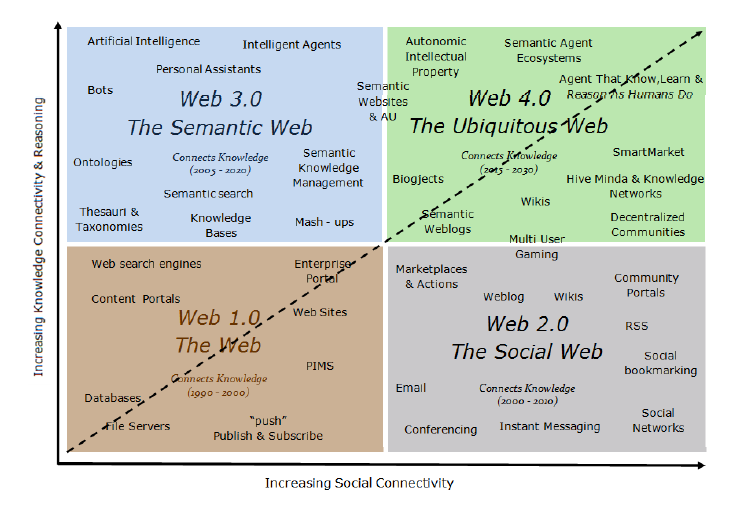
\includegraphics[width=11cm]{./imagenes/utilizacion_internet.png}
    \caption{Cambio de la utilización de internet en función de los servicios de conectividad social que son creados y soportados en ella}
    \label{fig:utilizacion_internet}
    \textbf{Fuente:}  http://goo.gl/3jGPPJ - Evolución de la web. Lozada, Pablo.
  \end{center}
\end{figure}


\section{Réd social}

La información contenida en la actual sección es tomada del libro \textit{Social Network Analisis for Startups} \cite{sna_startups}

Una red es un conjunto de relaciones. Mas específicamente, una red consiste en un conjunto de objetos (nodos) que están interconectados a través de relaciones (aristas). La red mas simple consiste en 2 nodos, N1 y N2, que están relacionados entre sí (Figura \ref{fig:simple}). Los nodos podrían representar personas, mientras la arista representa la relación que existe entre ellas (N1 y N2 son amigos, por ejemplo).

\begin{figure}[!htb]
  \begin{center}
    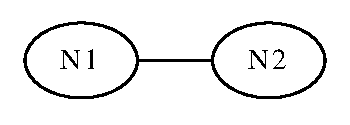
\includegraphics{./imagenes/Red_simple.eps}
    \caption{La red mas simple.}
    \label{fig:simple}
    \textbf{Fuente:}  Autores
  \end{center}
\end{figure}

Las redes sociales fuera de línea son las redes sociales que se forman por comunicación tradicional (lenguaje oral y escrito en medios que difieran de aquellos que utilizan las telecomunicaciones). Las redes sociales en línea son aquellas redes sociales que están formadas por cibernautas y en las cuales la comunicación se da por medio de los servicios de redes sociales. \cite{analysis}

Las relaciones pueden ser simétricas o asimétricas. Cuando se tiene una relación simétrica se dice que la relación no tiene dirección, es decir, la relación puede leerse en ambos sentidos. En el ejemplo anterior, significaría que N1 es amigo de N2 y que N2 es amigo de N1. Para que una relación se considere asimétrica, la relación debe poder leerse en un único sentido, es decir, la relación tiene una dirección determinada. En la figura \ref{fig:asimetrica} se puede observar un ejemplo de una red asimétrica en donde el nodo (o persona) N1 sigue al nodo N2, pero el nodo N2 no sigue al nodo N1.

\begin{figure}[!htb]
  \begin{center}
    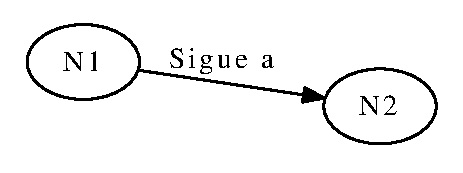
\includegraphics{./imagenes/Red_asimetrica.eps}
    \caption{Ejemplo de una red asimétrica.}
    \label{fig:asimetrica}
    \textbf{Fuente:}  Autores
  \end{center}
\end{figure}

Es posible que exista mas de una relación entre 2 nodos, en ese caso se dice que existe una \textit{relación multiplex} \cite[Cap.2]{cap_sna}


\section{Business Process Modeling Notation (BPMN)}

La información contenida en la actual sección es tomada del libro \textit{BPMN 2.0 Introduction to the Standard for Business Process Modeling} \cite{bpmn2}

Al interior de una organización es importante documentar y especificar los diferentes procesos que se deben llevar a cabo. A menudo, se suelen utilizar diagramas de flujo o incluso descripciones textuales. Desafortunadamente, estas técnicas se quedan cortas a la hora de describir procesos mas complejos, y mas aún cuando cada organización define su propia notación, dificultando el entendimiento de los diferentes modelos que se realizan al interior de la organización. Es por esto que se hace necesario crear una notación estándar y especifica para describir este tipo de procesos.

BPMN, Business Process Modeling Notation, es precisamente el estándar que se viene adoptando a nivel masivo para la creación y descripción de los diferentes procesos que hacen parte del funcionamiento de las diferentes organizaciones.


Con el estándar BPMN, se tienen en cuenta diferentes elementos básicos que sirven como herramientas para crear y estructurar los diferentes modelos que se quieran hacer. Estos elementos solo describen una forma básica de uso, pues BPMN permite personalizar los elementos a utilizar, siempre y cuando los cambios realizados no dificulten el proceso de entendimiento de los modelos.

\subsection{Pertinencia con el proyecto}

Se utilizará BPMN como ayuda para el modelamiento de los diferentes procesos de negocio que sean identificados en la fase de análisis. Esto facilitará el proceso de diseño e implementación de los diferentes componentes necesarios para dar solución a los diferentes requerimientos del negocio.

\section{Service-Oriented Architecture (SOA)}

La información contenida en la actual sección es tomada del libro \textit{Soa principles of service design} \cite{soa_principles}

\subsection{Primeros conceptos}

Los conceptos base del diseño de software deben ser expuestos para tener una mayor claridad en los temas siguientes. A continuación se expresan los conceptos base:

\begin{itemize}
  \item \textbf{Características de diseño}: Son aquellos atributos que cumple un diseño y que pueden ser medidos.
  \item \textbf{Principio de diseño}: Es una guía o regla para solucionar un problema de acuerdo a las prácticas aceptadas por la comunidad de ingeniería de software.
  \item \textbf{Paradigma de diseño}: Es el compendio de principios de diseño que tienen un enfoque global común.
  \item \textbf{Patrones de diseño}: Son formas de resolver un problema de diseño que es repetitivo. Viene dado por 3 restricciones presentadas en el diseño de software:
  \begin{itemize}
    \item Restricciones impuestas por la tecnología existente
    \item Restricciones impuestas por las tecnologías usadas por sistemas transversales
    \item Restricciones de prioridades de proyectos
  \end{itemize}
  El patrón de diseño describe el problema y da la solución a modo de plantilla.
  \item \textbf{Lenguajes de patrones de diseño}: Es la configuración ordenada de patrones en un diseño lógico. La comunicación entre cada patrón se hace a través de dicho lenguaje.
  \item \textbf{Estándares de diseño}: En orden de ir acorde a las metas, prioridades, recursos y ambiente de la organización en la que se haga el diseño lógico de la solución, un estándar de diseño define convenciones para cada elemento utilizado en el diseño de acuerdo a las características de diseño definidas.
  \item \textbf{Buenas prácticas}: Es una técnica o acercamiento para resolver o prevenir problemas presentados en el desarrollo del diseño lógico de la solución de software. pg 34
\end{itemize}

\begin{figure}[!htb]
  \begin{center}
    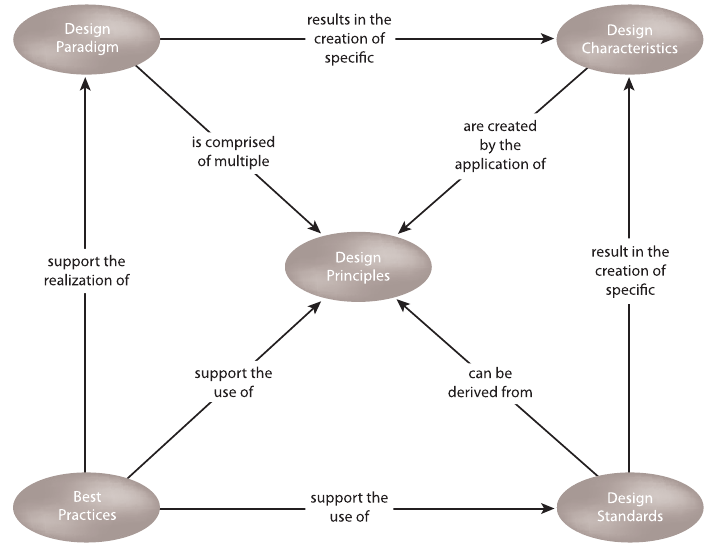
\includegraphics[width=11cm]{./imagenes/1.png}
    \caption{Acercamiento a cómo se desarrollan los principios de diseño con los demás conceptos nombrados.}
    \label{fig:uno}
    \textbf{Fuente:}  \cite{soa_principles}
  \end{center}
\end{figure}

La figura \ref{fig:uno} presenta un acercamiento a cómo se desarrollan los principios de diseño con los demás conceptos nombrados.

\begin{figure}[!htb]
  \begin{center}
    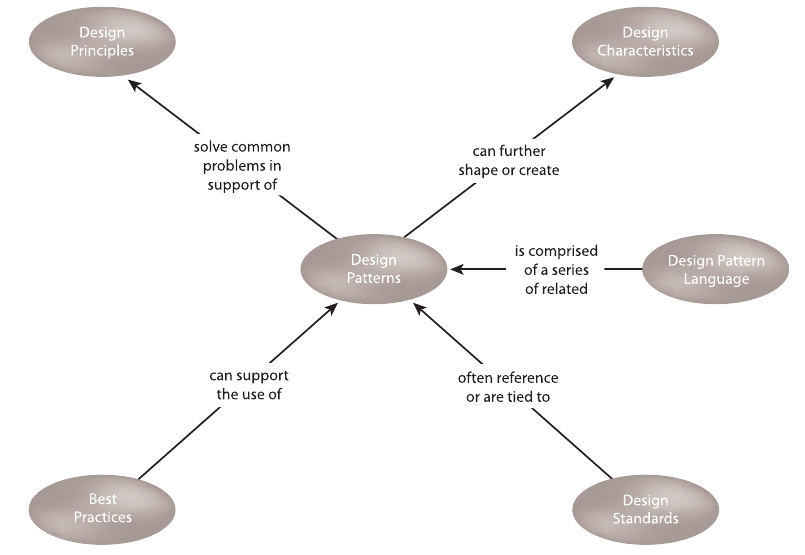
\includegraphics[width=11cm]{./imagenes/2.png}
    \caption{Como extiende o soporta un patrón de diseño el diseño lógico de la solución de software.}
    \label{fig:dos}
    \textbf{Fuente:}  \cite{soa_principles}
  \end{center}
\end{figure}

La figura \ref{fig:dos} presenta cómo extiende o soporta un patrón de diseño el diseño lógico de la solución de software.

\begin{figure}[!htb]
  \begin{center}
    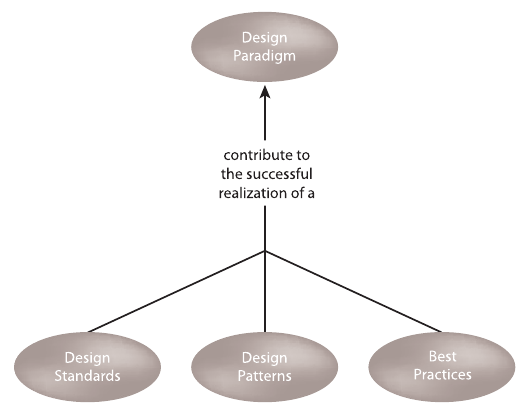
\includegraphics[width=11cm]{./imagenes/3.png}
    \caption{Componentes que hacen que el diseño lógico de la solución sea acorde al paradigma escogido.}
    \label{fig:tres}
    \textbf{Fuente:}  \cite{soa_principles}
  \end{center}
\end{figure}

La figura \ref{fig:tres} presenta los componentes que hacen que el diseño lógico de la solución sea acorde al paradigma escogido.

\subsection{Computación orientada a servicios}

La computación orientada a servicios nace de la necesidad de desarrollar software integrado con otros construidos con diferentes arquitecturas y, por ende, diversas tecnologías. Este tipo de computación tiene como finalidad la construcción de inventarios de servicios. La computación orientada a servicios está compuesta por la interacción de la orientación a servicios (paradigma de diseño) y la arquitectura orientada a servicios, formando patrones de diseño propios y estándares en cumplimiento de las características de diseño propias de la computación orientada a servicios. 

Algunos de los conceptos clave llevados en la computación orientada a servicios son:

\begin{itemize}
  \item Arquitectura Orientada a Servicios (SOA - Service Oriented Architecture): Comprende el compendio de tecnologías, APIs, infraestructura y repositorios enmarcados en el paradigma orientado a servicios y cuyo objetivo principal es el de trabajar sobre el "servicio" como el elemento más importante.
  \item Orientación a servicios: Es el paradigma manejado en la computación orientada a servicios en donde se acepta como unidad mínima y más importante el "servicio".
  \item Servicio: Es un software independiente físicamente el cual tiene asignado un contexto de funcionalidades y que puede ser utilizado por otros servicios por medio del contrato del servicio (descripción del servicio en cuanto a funcionalidades, entradas requeridas y salidas). De acuerdo a su nivel de reúso, los servicios se dividen en 3 tipos y son:
  \begin{itemize}
    \item Servicios entidad: Modela los servicios que se deben ofrecer respecto de las entidades del negocio (ej. empleados y clientes). Tienen un nivel de reúso alto y están centrados en el negocio.
    \item Servicios tarea: Modela los servicios que deben cumplir tareas específicas del negocio (ej. generación de cortes de final de año). Tienen un nivel de reúso bajo. Estos servicios trabajan directamente con 1 o varios servicios entidad. Estos servicios están centrados en el negocio.
    \item Servicios utilidad: Modela servicios que no están centrados en el negocio. Son los servicios con mayor reúso.
  \end{itemize}
\end{itemize}

\begin{figure}[!htb]
  \begin{center}
    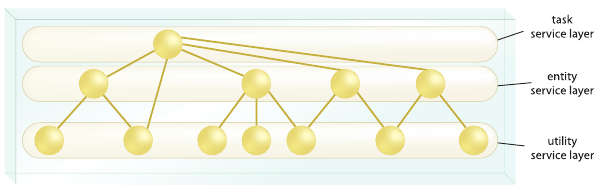
\includegraphics[width=11cm]{./imagenes/5.png}
    \caption{diferenciación entre tipos de servicio da lugar a la estructura en capas}
    \label{fig:cinco}
    \textbf{Fuente:}  \cite{soa_principles}
  \end{center}
\end{figure}

La diferenciación entre tipos de servicio da lugar a la estructura en capas mostrada en la figura \ref{fig:cinco}

\begin{itemize}
  \item Composición de servicios: Es la agregación de servicios de manera ordenada.
  \item Inventario de servicios: Es la agrupación de varios servicios según un criterio definido por la organización. Cada inventario de servicios tiene su propio estándar de diseño e, inclusive, su propia configuración arquitectónica. El desarrollo de los inventarios de servicio es hecho a modo top-down, con la construcción de blueprints, también llamados modelo de servicios de negocio o modelos de inventario de servicios.
\end{itemize}

\begin{figure}[!htb]
  \begin{center}
    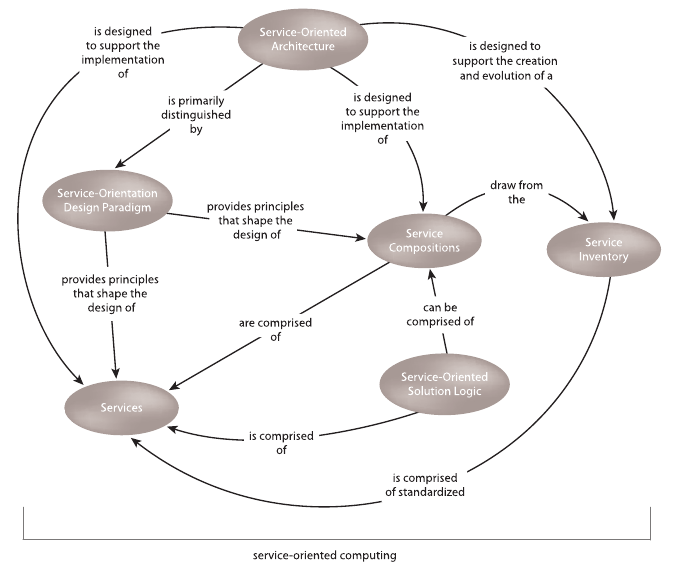
\includegraphics[width=11cm]{./imagenes/4.png}
    \caption{Interacción de los conceptos clave en la computación orientada a servicios}
    \label{fig:cuatro}
    \textbf{Fuente:}  \cite{soa_principles}
  \end{center}
\end{figure}

\subsection{Pertinencia con el proyecto}


La arquitectura base para la ejecución del proyecto es SOA. Esto brinda diferentes beneficios a la hora del desarrollo del proyecto, como los son:
\begin{itemize}
  \item Gracias al bajo acoplamiento conseguido con la arquitectura SOA, los componentes implementados son altamente reutilizables, lo que facilita y agiliza el proceso de desarrollo. Ademas,
  \item Es posible consumir servicios creados por terceros, limitando los servicios que deben ser creados a los que sean estrictamente de negocio.
\end{itemize}

\section{Scrum}

Sus creadores lo describen como “Un marco de trabajo por el cual las personas pueden acometer problemas complejos 
adaptativos, a la vez que entregar productos del máximo valor posible productiva y creativamente” \cite{scrum_guide}. Scrum se caracteriza por ser ágil, ligero, fácil de entender y difícil de llegar a dominar.

Scrum se basa en el empirismo, que dice que el conocimiento proviene de la experiencia, por lo que ``utiliza un enfoque iterativo e incremental para optimizar la predictibilidad y el control del riesgo'' \cite{scrum_guide}.

Los tres grandes pilares de la teoría de scrum son:

\begin{itemize}
  \item Transparencia: Todos los aspectos significativos deben ser visibles para sus stakeholders respectivos.

  \item Inspección: Los artefactos de scrum (y su progreso) deben ser inspeccionados frecuentemente para detectar variaciones. Estas inspecciones deben ser realizadas por un experto.

  \item Adaptación: Cuando una inspección detecta una variación que no cae en los limites permitidos, se deben hacer los reajustes necesarios para que el producto vuelva a rumbo deseado. Estos cambios deben hacerse lo más pronto posible, por esto las inspecciones deben ser realizadas de manera periódica a lo largo del desarrollo del proyecto.
\end{itemize}

 
  \chapter{Marco teórico}
  \section{Redes Sociales} \label{sec:red}

La información contenida en la actual sección es tomada del libro \textit{Social Network Analisis for Startups} \cite{sna_startups}

\subsection{SNA: Social Network Analisis}

La administración de una red social fuera de línea fue estudiada desde inicios del siglo XX \cite{dynamics} con un enfoque socio-matemático llamado “análisis de redes sociales” (SNA por sus siglas en inglés: Social Network Analisis). Sin embargo, era difícil el análisis del comportamiento humano según los designios de la SNA, puesto que la información debía ser recopilada por medio de entrevistas a las personas. Aun así, el enfoque SNA fue utilizado para analizar el comportamiento terrorista o inclusive el comportamiento de trabajadores en una empresa. \cite{sna_startups}

\subsection{Analisis egocéntrico} \label{sec:egocentrico}

Los estudios basados en SNA pueden ser de tipo egocéntrico o sociocéntrico \cite{user_behavior}. En los estudios egocéntricos de una red social, se analiza un individual dentro de una red social y todas las conexiones de éste hacia otros individuales en la red social analizada. El individual analizado es llamado “ego” y los individuales que hacen conexión con él son llamados “alters”. Se han identificado 4 capas en el estudio de las redes egocéntricas, estas son:

\begin{itemize}
  \item Support clique: En esta capa se identifican los alters con los que el ego hace más contacto por alguna razón de peso para él (e.g. para obtener soporte emocional). Esta capa tiene, en promedio, 5 alters.
  \item Sympathy group: En promedio a éste corresponden 15 alters.
  \item Affinity group: En promedio a éste corresponden 50 alters.
  \item Active network: En promedio a éste corresponden 150 alters.
\end{itemize}

Los números dados en las capas descritas en el análisis egocéntrico son congruentes con el número de Dunbar, el cual representa el umbral promedio de número de alters sobre la capa “active network” (150) según Robin Dunbar, argumentando que este límite se debe a la capacidad cognitiva del cerebro humano \cite[Pag. 3]{dynamics} (como más adelante será nombrado, los servicios de redes sociales ayudan al ser humano a gestionar su active network, proporcionando herramientas que, en teoría y de acuerdo a la brecha tecnológica, lo ayudarán a mantener sus lazos con los alters de su red ego).

El análisis egocéntrico permite conocer los factores que dirigen al ego a crear vínculos débiles o fuertes con potenciales alters, albergándolos en alguna de las cuatro capas o en ninguna.

Con la creación de las OSN y la gran cantidad de información que describe el comportamiento humano sobre este tipo de red social, ha sido más sencillo utilizar el enfoque de la SNA para estudiar que comportamientos tienen los humanos sobre una red social establecida.

\subsection{Grado de centralidad}

En todas las redes, sean virtuales o no, existen personas que son mas ``importantes'' que otras, más \textbf{populares}. Estas celebridades representan una parte muy pequeña de la red, pero debido a su gran influencia siempre es bueno identificarlos. Para esto se utiliza el \textbf{grado de centralidad}.

El grado de un nodo es la cantidad de conexiones que posee. En una red social, esto se representa por medio de las relaciones que cada nodo tenga, y ya que el significado de la relación varía en función de cada red, es necesario entender que significan las posibles relaciones existentes en una red para hacer el análisis correspondiente. Por ejemplo, en una red como Twitter en donde las relaciones son unidireccionales, puede existir un nodo con un grado de salida muy alto, esto es una persona que sigue a muchas otras. Aunque esta persona tenga un grado de centralidad muy alto, no representa una celebridad, sin embargo, un nodo que tenga un grado de entrada muy alto, que es seguido por muchas personas, si representa una persona que es muy popular en esta red.

\begin{figure}[!htb]
  \begin{center}
    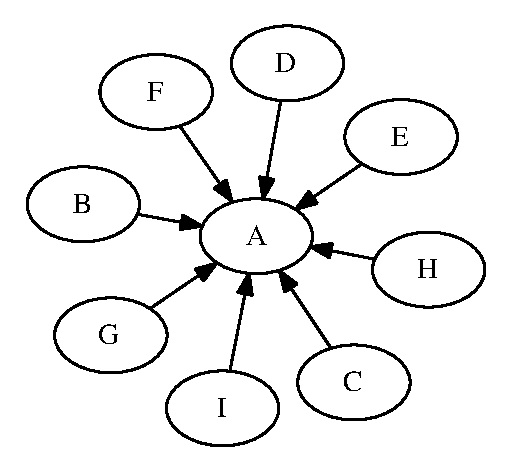
\includegraphics{./imagenes/red_estrella.eps}
    \caption{Red de estrella.}
    \label{fig:red_estrella}
    \textbf{Fuente:}  Autores
  \end{center}
\end{figure}


En la figura \ref{fig:red_estrella} se puede ver un caso en el que el nodo A es una clara celebridad de la red. Este tipo de configuración, llamada red de estrella, es muy poco común en la vida real, pero sirve de ayuda visual para entender a simple vista el concepto de centralidad.

\subsection{Grado de cercanía}

A menudo se puede ver que personas que no tienen mayor influencia aparente en una red son capaces de difundir un mensaje en una gran parte de la red. Esto se debe a que tienen buenas conexiones en la red que les permiten llegar a mas personas, sin que ellos en si sean ``importantes'' en la red. Para medir que tan bien o mal posicionado esta un nodo en la red se utiliza el \textbf{grado de cercanía}. Este calculo es bastante caro computacionalmente ya que conlleva una gran cantidad de cálculos.

Los pasos para calcular el grado de cercanía de los nodos de una red son:

\begin{enumerate}
  \item Calcular la ruta mas corta entre todos los pares de nodos posibles, utilizando el algoritmo de Dijkstra, y almacenar estos valores en una tabla.
  \item Para cada nodo de la red:
  \begin{enumerate}
    \item Calcular la distancia promedio con todos los demás nodos.
    \item Dividir el promedio por la distancia mas alta.
    \item Calcular el inverso del valor anterior.
  \end{enumerate}
  \item normalizar cada valor obtenido para obtener valores en el rango de 0-1.
\end{enumerate}

Los nodos que tengan un valor mas cercano a 1 son los que tienen una distancia promedio menor con los nodos de la red, o los que tienen ``\textit{mejores contactos}''.

\subsection{Factor distancia en la formación de las redes sociales}

La formación de redes sociales (tanto fuera de línea como en línea) es afecta por la distancia entre cada individual y el posible tipo de enlace que los uniría. En \cite{evolution} se hizo un estudio acerca de la formación de lazos, la formación de triadas entre individuales de una red social basada en la inscripción localizaciones recomendadas y frecuentadas por los usuarios, teniendo como parámetros ``la edad'' o tiempo de vinculación del individual a la red social, el grado de cada individual (número de conexiones que tiene un individual a otro) y la localización de cada individual en la red social. También se analizó cómo afectaba la creación de nuevos lazos con la movilidad del usuario (el desplazamiento por lugares geográficos distintos). En conclusión, se verificó que la formación de lazos depende proporcionalmente de la edad y del grado del individual y es inversamente proporcional a la distancia que a cada individual y que la formación de lazos puede modelarse con solo dos de los tres factores (el grado y la distancia); en cuanto a la formación de triadas, se verificó que ésta depende de las características sociales de la red, tomando énfasis en los individuales compartidos entre los posibles individuales formadores de triadas. Además, en cuanto a la creación de nuevos lazos teniendo en cuenta los lugares visitados por cada usuario de la red social, se presenta un patrón: Los usuarios escogen un lugar popular para visitar y, posteriormente, dirimen con que usuario crear un lazo teniendo en cuenta su popularidad y que frecuente los mismos lugares siempre.

\subsection{Grado de intermediación}

En las redes sociales, suelen formarse grupos mas pequeños que comparten un interés común. Por ejemplo, es mas probable que dos personas que comparten el gusto por los videojuegos interactúen entre si que dos personas que no lo hagan, sin embargo hay casos en los que una persona comparte gustos con diferentes grupos, ayudando a que esta persona se pueda relacionar de manera efectiva con un grupo mas extenso de personas. Estas personas son conocidas como ``puertas frontera'' ya que, gracias a ellos, es posible que dos grupos que no tengan nada en común puedan relacionarse entre sí. La medida que ayuda a identificar estos elementos en una red es el \textbf{grado de intermediación}, y consiste en lo siguiente:

\begin{enumerate}
  \item Calcular la ruta mas corta entre todos los pares de nodos posibles, utilizando el algoritmo de Dijkstra, y almacenar estos valores en una tabla.
  \item Para cada nodo n de la red, contar las veces que el nodo n aparece en la lista de rutas mas cortas,
  \item normalizar cada valor obtenido para obtener valores en el rango de 0-1.
\end{enumerate}

Cabe notar que este algoritmo es bastante lento para redes que son muy grandes.

En la figura \ref{fig:bow_tie} se puede ver un claro ejemplo de este fenómeno. Esta red, comúnmente denominada la "red corbatín" gracias a su forma similar a la de un corbatín, muestra como el nodo D se encuentra entre 2 grupos de nodos que, de otra manera, no podrían conectarse.

\begin{figure}[!htb]
  \begin{center}
    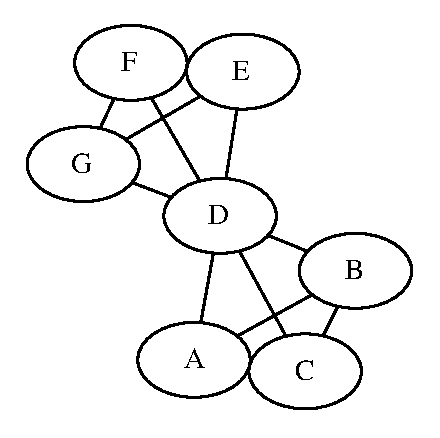
\includegraphics{./imagenes/bow_tie.eps}
    \caption{red corbatín.}
    \label{fig:bow_tie}
    \textbf{Fuente:}  Autores
  \end{center}
\end{figure}

\subsection{Díadas}

Las díadas son la unidad básica de análisis una red social, ya que estas representan la relación entre una y otra persona, esto es, mis amigos, mis seguidores, mis suscriptores, etc. Existen 4 tipos de díadas, representadas en la figura \ref{fig:tipos_diadas}, su uso varia en función del significado de la relación.

\begin{figure}[!htb]
  \begin{center}
      \begin{tabular}{m{3cm}|m{3cm}|m{3cm}|m{3cm}}
        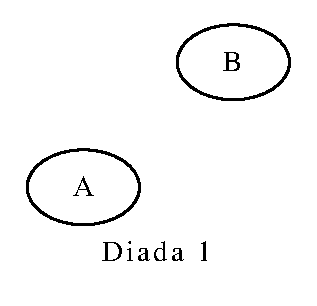
\includegraphics[width=3cm]{./imagenes/diada_1.eps} & 
        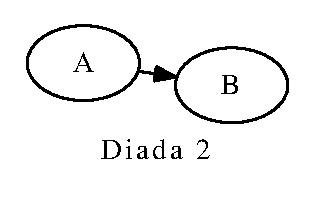
\includegraphics[width=3cm]{./imagenes/diada_2.eps} & 
        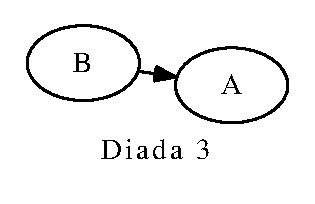
\includegraphics[width=3cm]{./imagenes/diada_3.eps} & 
        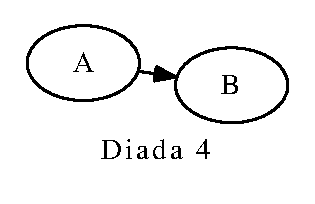
\includegraphics[width=3cm]{./imagenes/diada_4.eps}\\
      \end{tabular}
    \caption{Tipos de diadas asimétricas.}
    \label{fig:tipos_diadas}
    \textbf{Fuente:}  Autores
  \end{center}
\end{figure}


La díada 1 indica que ambos individuos existen en la red, pero todavía no existe ninguna relación entre ellos. Las diadas 2 y 3 muestran una relación unidireccional entre los dos individuos, la única diferencia es el sentido de esa relación. La díada 4, por su parte, es la de mayor interés de las cuatro ya que muestra una relación bidireccional entre los individuos, siendo esta la relación que mayor peso tiene en una red social dado que nos dice que existe un alto grado de reciprocidad en el intercambio de información entra ambos individuos.

\subsection{Tríadas}

Las triadas son básicamente 3 nodos conectados de alguna manera. Al igual que con las diadas, las triadas también pueden ser simétricas o asimétricas, dependiendo estrictamente del contexto en que son utilizadas. Existen 4 tipos de triadas simétricas, ilustradas en la figura \ref{fig:tipos_triadas_simetricas}.

\begin{figure}[!htb]
  \begin{center}
      \begin{tabular}{m{3cm}|m{3cm}|m{3cm}|m{3cm}}
        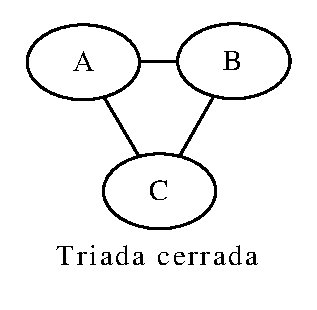
\includegraphics[width=3cm]{./imagenes/triada_simetrica_1.eps} & 
        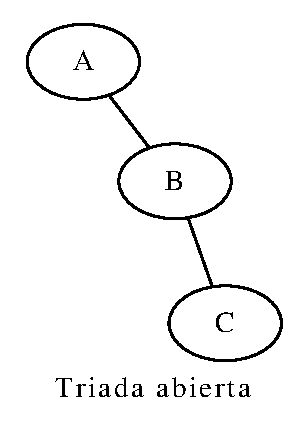
\includegraphics[width=3cm]{./imagenes/triada_simetrica_2.eps} & 
        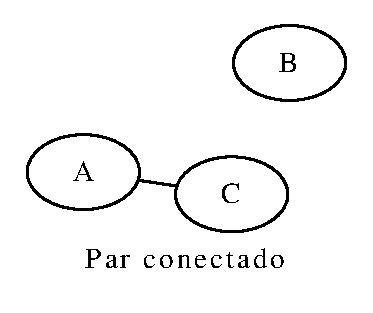
\includegraphics[width=3cm]{./imagenes/triada_simetrica_3.eps} & 
        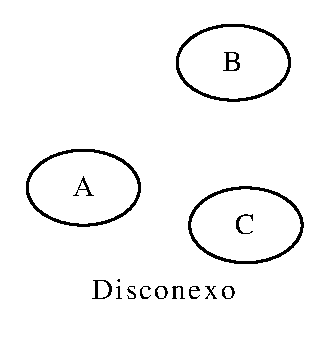
\includegraphics[width=3cm]{./imagenes/triada_simetrica_4.eps}\\
      \end{tabular}
    \caption{Tipos de triadas simétricas.}
    \label{fig:tipos_triadas_simetricas}
    \textbf{Fuente:}  Autores
  \end{center}
\end{figure}


Por otra parte, existen 16 tipos de triadas asimétricas, numeradas del 1-16. Su uso es mas frecuente ya que de ellas se puede hacer un análisis mas complejo en comparación a las díadas. Cada una de estas triadas recibe un nombre especifico para facilitar su identificación, a continuación se explica como debe leerse ese nombre:

\begin{itemize}
  \item El primer numero representa la cantidad de vértices bidireccionales
  \item El segundo numero representa la cantidad de vértices simples
  \item El tercer numero representa la cantidad de vértices inexistentes
  \item Si una triada se repite, se utiliza una letra extra para determinar que variante es:
  \begin{itemize}
    \item U - Arriba (Up)
    \item D - Abajo (Down)
    \item C - Circulo (Circle)
    \item T - Transitiva (Transitive)
  \end{itemize}
\end{itemize}

En la figura \ref{fig:tipos_triadas_asimetricas} se muestran todas las triadas posibles con su respectivo código asociado.

\begin{figure}[!htb]
  \begin{center}
      \begin{tabular}{m{1.3cm}|m{1.3cm}|m{1.3cm}|m{1.3cm}|m{1.3cm}|m{1.3cm}|m{1.3cm}|m{1.3cm}}
        \includegraphics[width=1.3cm]{./imagenes/triada_003.eps} & 
        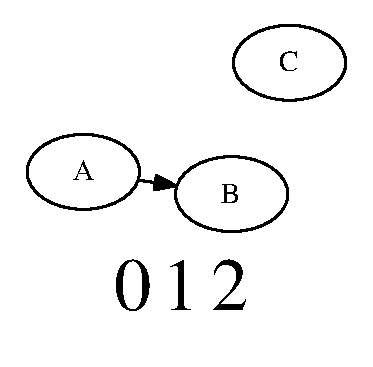
\includegraphics[width=1.3cm]{./imagenes/triada_012.eps} & 
        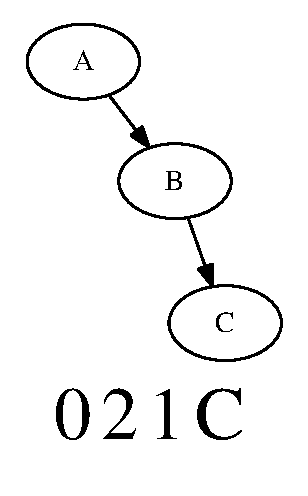
\includegraphics[width=1.3cm]{./imagenes/triada_021C.eps} & 
        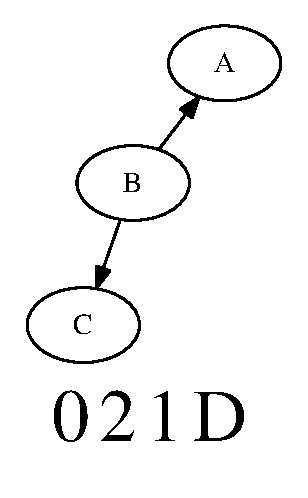
\includegraphics[width=1.3cm]{./imagenes/triada_021D.eps} & 
        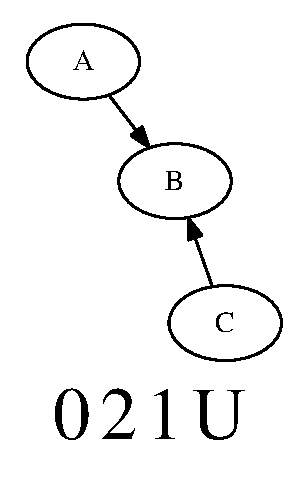
\includegraphics[width=1.3cm]{./imagenes/triada_021U.eps} & 
        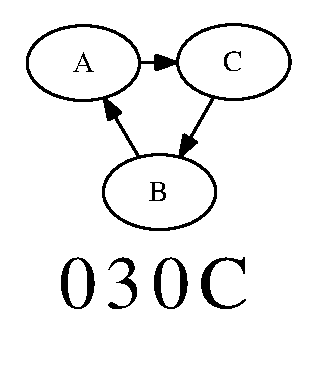
\includegraphics[width=1.3cm]{./imagenes/triada_030C.eps} & 
        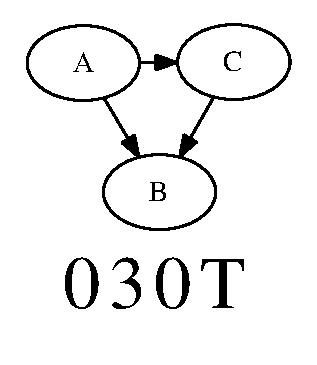
\includegraphics[width=1.3cm]{./imagenes/triada_030T.eps} & 
        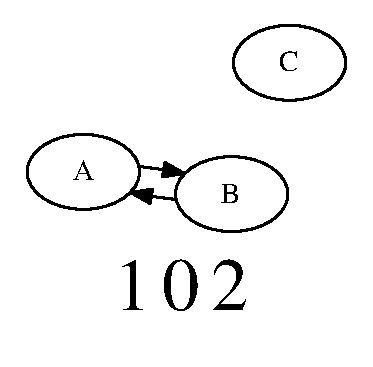
\includegraphics[width=1.3cm]{./imagenes/triada_102.eps}\\ \hline
        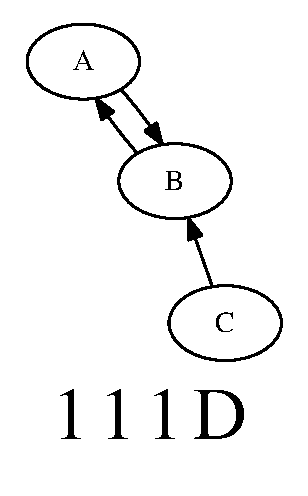
\includegraphics[width=1.3cm]{./imagenes/triada_111D.eps} & 
        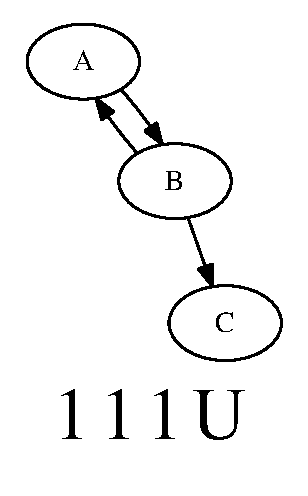
\includegraphics[width=1.3cm]{./imagenes/triada_111U.eps} & 
        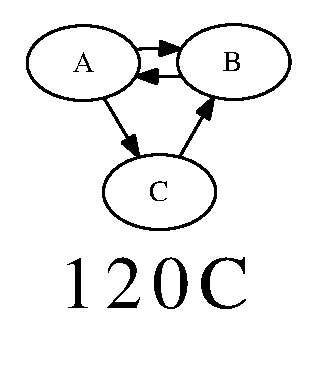
\includegraphics[width=1.3cm]{./imagenes/triada_120C.eps} & 
        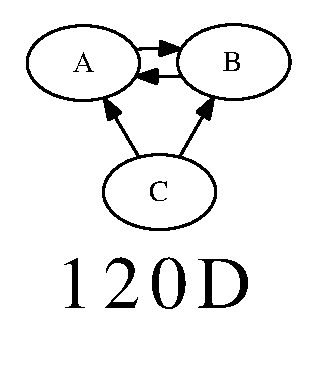
\includegraphics[width=1.3cm]{./imagenes/triada_120D.eps} & 
        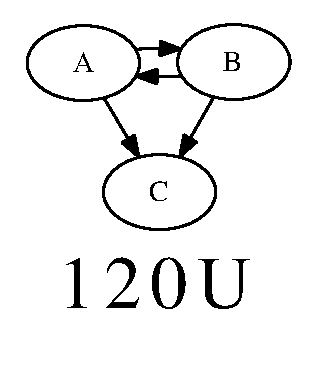
\includegraphics[width=1.3cm]{./imagenes/triada_120U.eps} & 
        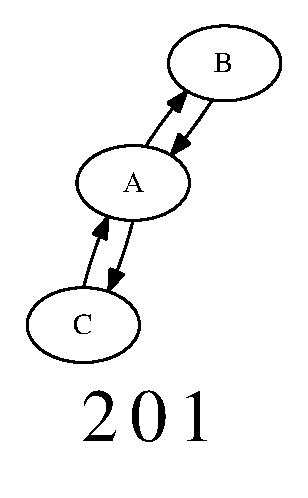
\includegraphics[width=1.3cm]{./imagenes/triada_201.eps} & 
        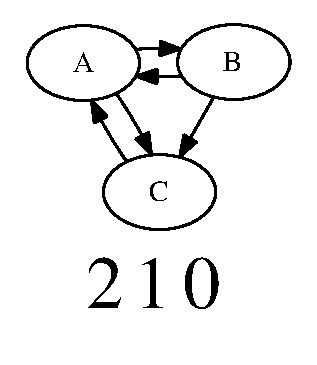
\includegraphics[width=1.3cm]{./imagenes/triada_210.eps} & 
        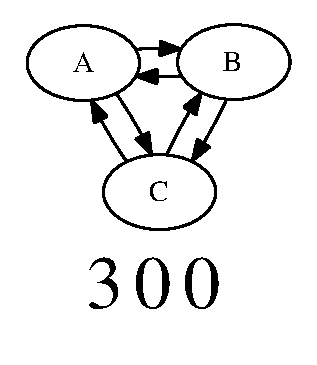
\includegraphics[width=1.3cm]{./imagenes/triada_300.eps}\\
      \end{tabular}
    \caption{Tipos de triadas asimétricas.}
    \label{fig:tipos_triadas_asimetricas}
    \textbf{Fuente:}  Autores
  \end{center}
\end{figure}


Gracias a esta discriminación topológica, se puede hacer un análisis mas completo de una red. Este análisis recibe el nombre de \textbf{\textit{Análisis Triadico}}.

\subsection{Análisis Triádico}

Este proceso, que también recibe el nombre de \textbf{Censo Triadico}, consiste en contar la ocurrencia de cada uno de los tipos de triada para cada nodo, y de esa forma determinar el rol que desempeña este nodo en la red. Por ejemplo, un nodo que presente en mayoría triadas del tipo 4, 7 y 11 es un nodo que \textbf{genera contenido}, mientras que si la mayoría de sus triadas son del tipo 5 y/o 10, es un nodo que recibe o \textbf{consume contenidos}.

Adicionalmente se puede hacer el mismo análisis a la red en general, para tener un punto de vista global de la red. En la figura \ref{fig:red_krackhardt} se puede ver una de las redes mas utilizadas en la teoría de redes sociales, la red de Krackhardt-kite. En esta red se pueden ver muchas características de una red social, facilitando el estudio de las mismas. Al hacer el censo a esta red, nos damos cuenta que presenta una gran cantidad de nodos tipo 201, que representan un agujero estructural, y nodos tipo 300, que representan triadas cerradas, esto nos indica que en esta red existen zonas que tienen una gran concentración de nodos interconectados, mientras hay zonas que no se encuentran muy pobladas. Todo esto se puede ver a simple vista en esta red, pero para redes mas grandes puede que represente un problema mayor.

\begin{figure}[!htb]
  \begin{center}
    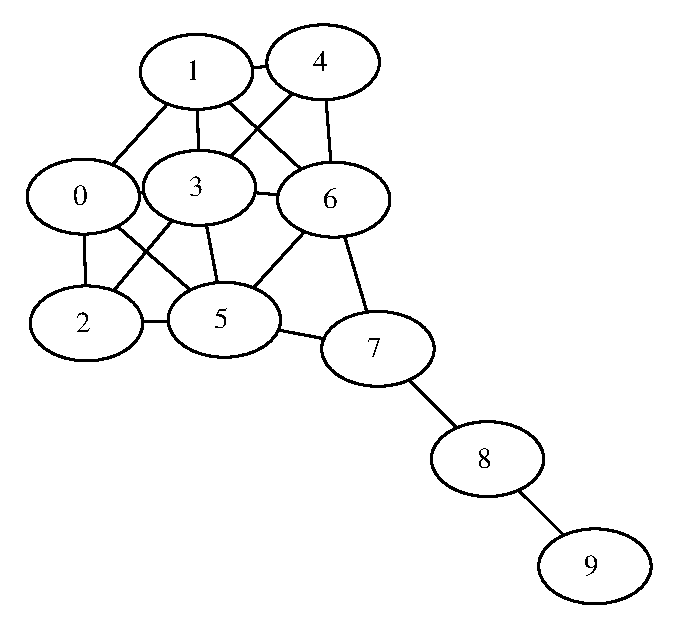
\includegraphics[width=8cm]{./imagenes/red_krackhardt_kite.eps}
    \caption{Red social de Krackhardt kite.}
    \label{fig:red_krackhardt}
    \textbf{Fuente:}  Autores
  \end{center}
\end{figure}



\section{UX - Análisis} \label{sec:UX}
Los servicios de redes sociales (SNS por sus siglas en ingles: Social Network Services) como Facebook, LinkedIn, Twitter, SportTracker o Xportia, ofrecen servicios para la gestión de la OSN de cada usuario que acceda a estas aplicaciones. Según un estudio hecho para medir la experiencia de usuario \cite{user_behavior_online} (UX por sus siglas en ingles: User eXperience) en los SNS, se encontraron 8 categorías que son críticas a la hora de diseñar una SNS y son:

\begin{enumerate}
  \item Self-expresion: Capacidad que tengan las OSN de compartir contenido relacionado a la vida real de los usuarios tal como lo pueden ser las fotos, los videos, los comentarios o las comunicaciones directas.
  \item Reciprocity: Interacción bilateral en tiempo real, es decir, interacción instantánea con uno o varios individuales en la OSN (por ejemplo, por medio de los servicios de mensajería instantánea).
  \item Learning: La información recibida por medio de la OSN debe poder ser utilizada en pro del desarrollo cognitivo del individual; debe existir información útil al individual que usa la OSN.
  \item Curiosity: El contenido de la OSN debe ser interesante para quien la utiliza.
  \item Suitability of functionality: Se refiere a cuán ``utilizable'' es una funcionalidad.
  \item Suitability of content: La calidad y exactitud de la información que en la OSN reside debe ser suficiente para el individual perteneciente a ella.
  \item Completeness of the user network: Los individuales deben querer pertenecer a la red social y buscar eficientemente a otros individuales para poder formar lazos con ellos y hacer crecer su red social.
  \item Trust and privacy: Confianza en los servicios de las OSN, así como también la capacidad que tiene el usuario de gestionar la privacidad del contenido que comparte en dicha OSN. \cite{social_experience}
\end{enumerate}

Cada uno de las categorías nombradas hace parte de los factores que impulsan la utilización de los SNS para la gestión de las OSN de las personas.


%\section{Business Process Modeling Notation (BPMN)}

La información contenida en la actual sección es tomada del libro \textit{BPMN 2.0 Introduction to the Standard for Business Process Modeling} \cite{bpmn2}

A continuación, se enuncian algunos conceptos básicos de BPMN.

\subsection{Enlaces}

Los enlaces sirven para unir o bifurcar el flujo de secuencia de un modelo. Son utilizadas cuando es necesario tomar algún tipo de decisión que lleve a tomar uno o varios caminos alternos. Existen varios tipos de enlaces, como lo son los enlaces exclusivos (XOR), paralelos (AND), inclusivos (OR) y complejos. A continuación, se muestran ejemplos de aplicación de cada uno de estos enlaces.

\begin{figure}[!htb]
  \begin{center}
    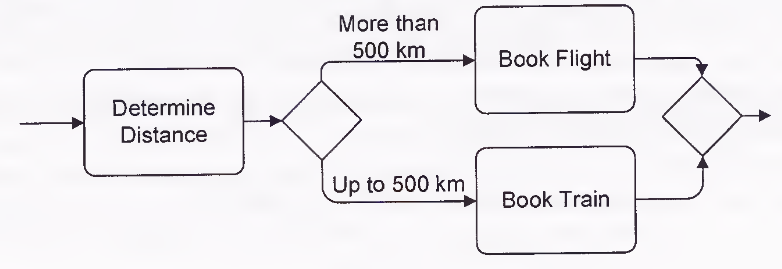
\includegraphics[width=11cm]{./imagenes/gateway_exclusivo.png}
    \caption{Ejemplo de uso del enlace exclusivo}
    \label{fig:gateway_exclusivo}
    \textbf{Fuente:}  \cite{bpmn2}
  \end{center}
\end{figure}

En este caso (Figura \ref{fig:gateway_exclusivo}), se realiza la actividad \textit{Determinar distancia} y se decide que tipo de medio de transporte se debe utilizar. Nótese que luego de realizar la reserva, se vuelve a unir el flujo de secuencia del modelo, ya que no se sabe en la práctica cual de las 2 alternativas será la seleccionada.

\begin{figure}[!htb]
  \begin{center}
    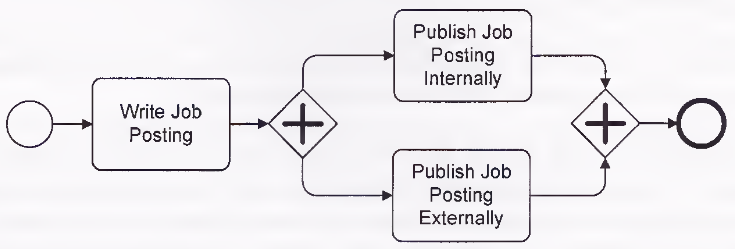
\includegraphics[width=11cm]{./imagenes/gateway_paralelo.png}
    \caption{Ejemplo de uso del enlace paralelo}
    \label{fig:gateway_paralelo}
    \textbf{Fuente:}  \cite{bpmn2}
  \end{center}
\end{figure}

En la figura \ref{fig:gateway_paralelo} se ve un ejemplo de uso de este enlace. Aquí, luego de que se redacta la oferta de trabajo, le procede a publicarla, tanto interna como externamente. En este caso, se utiliza el enlace paralelo para agilizar el proceso de publicación.

\begin{figure}[!htb]
  \begin{center}
    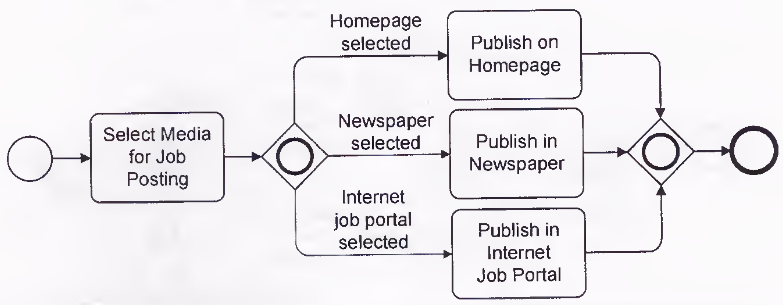
\includegraphics[width=11cm]{./imagenes/gateway_inclusivo.png}
    \caption{Ejemplo de uso del enlace inclusivo}
    \label{fig:gateway_inclusivo}
    \textbf{Fuente:}  \cite{bpmn2}
  \end{center}
\end{figure}


En la figura \ref{fig:gateway_inclusivo} se ve un ejemplo de uso en donde a partir de la actividad ``Seleccionar medio para publicar oferta de trabajo'' se pueden seleccionar una o varias opciones. Cualquier combinación de opciones, que al menos contenga una opción, es válida.

\begin{figure}[!htb]
  \begin{center}
    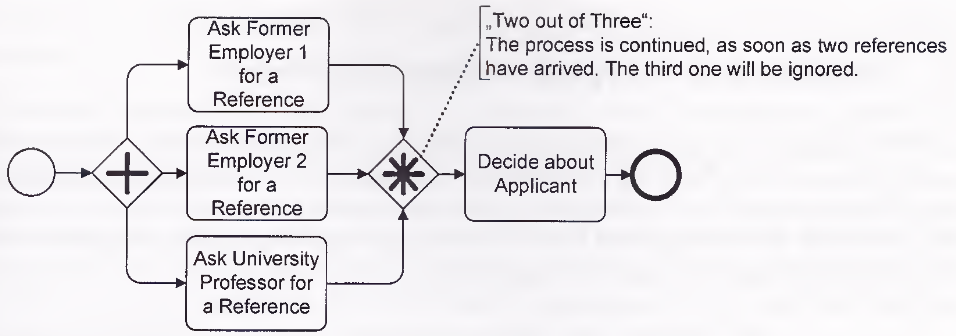
\includegraphics[width=11cm]{./imagenes/gateway_complejo.png}
    \caption{Ejemplo de uso del enlace complejo}
    \label{fig:gateway_complejo}
    \textbf{Fuente:}  \cite{bpmn2}
  \end{center}
\end{figure}


En el ejemplo mostrado en la figura \ref{fig:gateway_complejo}, se requiere la referencia de 2 empleadores previos y de la universidad. En realidad, solo son necesarias dos referencias, pero para estar seguros se piden tres, por lo que tan pronto como llegan las primeras 2 referencias, la tercera puede ser ignorada sin mayor problema.

\subsection{Colaboración}

A menudo, en un proceso intervienen diferentes partes interesadas ({\textit{Stakeholders}) y es necesario ver el proceso de manera global, de manera que el paso de mensajes entre las partes implicadas sea mas claro. A este tipo de diagramas se les llama \textbf{diagrama de colaboración}

La figura \ref{fig:diagrama_colaboracion} muestra como es la interacción entre un aspirante y una empresa en el proceso de acceder a una oferta de empleo. Puede verse como, entre las actividades que ejecuta cada una de las partes, existe un paso de mensaje que une ambos procesos. Esta unión se representa por una flecha con linea punteada, donde un extremo tiene un circulo y el otro una flecha vacía que indica la dirección del mensaje.

\begin{figure}[!htb]
  \begin{center}
    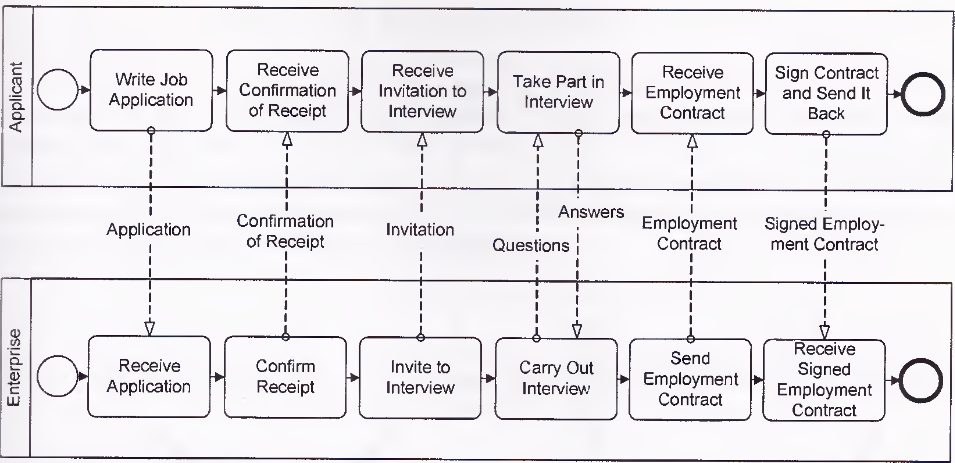
\includegraphics[width=11cm]{./imagenes/diagrama_colaboracion.png}
    \caption{Ejemplo de diagrama de colaboración}
    \label{fig:diagrama_colaboracion}
    \textbf{Fuente:}  \cite{bpmn2}
  \end{center}
\end{figure}


Por ejemplo, la actividad ``Recibir solicitud'' recibe un mensaje de la actividad ``Redactar solicitud de empleo'', por lo cual esta actividad (recibir solicitud) no puede iniciar si el aspirante no envía su solicitud. Esto significa que los mensajes deben ser respetados y una actividad no puede realizarse si le falta algún mensaje de entrada.

Sin embargo, en estos casos solo se conoce el proceso que sigue la empresa, por lo que es común representar a las partes externas como una caja negra (figura \ref{fig:diagrama_colaboracion_caja_negra}).

\begin{figure}[!htb]
  \begin{center}
    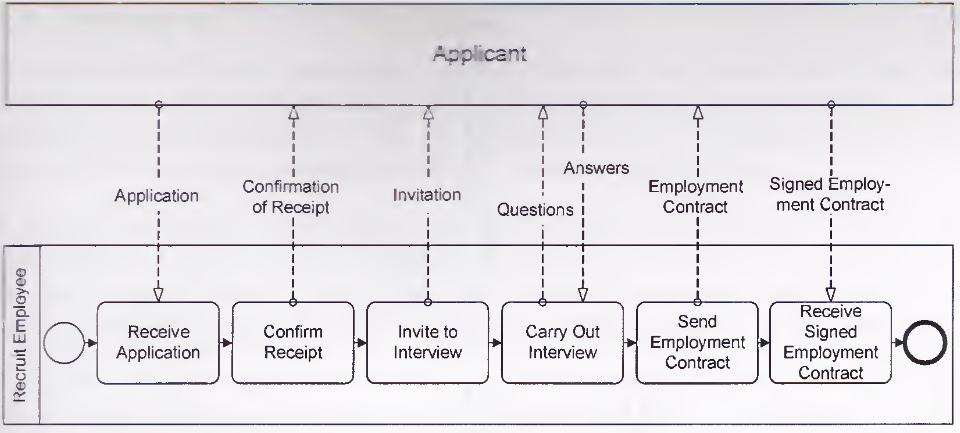
\includegraphics[width=11cm]{./imagenes/diagrama_colaboracion_caja_negra.png}
    \caption{Ejemplo de diagrama de colaboración con caja negra}
    \label{fig:diagrama_colaboracion_caja_negra}
    \textbf{Fuente:}  \cite{bpmn2}
  \end{center}
\end{figure}


\section{SOA}
\subsection{Primeros conceptos}

Los conceptos base del diseño de software deben ser expuestos para tener una mayor claridad en los temas siguientes. A continuación se expresan los conceptos base:

\begin{itemize}
  \item Características de diseño: Son aquellos atributos que cumple un diseño y que pueden ser medidos

  \item Principio de diseño: Es una guía o regla para solucionar un problema de acuerdo a las prácticas aceptadas por la comunidad de ingeniería de software.

  \item Paradigma de diseño: Es el compendio de principios de diseño que tienen un enfoque global común.

  \item Patrones de diseño: Son formas de resolver un problema de diseño que es repetitivo. Viene dado por 3 restricciones presentadas en el diseño de software:
  \begin{itemize}
    \item Restricciones impuestas por la tecnología existente
	  \item Restricciones impuestas por las tecnologías usadas por sistemas transversales
	  \item Restricciones de prioridades de proyectos
  \end{itemize}
  El patrón de diseño describe el problema y da la solución a modo de plantilla.

  \item Lenguajes de patrones de diseño: Es la configuración ordenada de patrones en un diseño lógico. La comunicación entre cada patrón se hace a través de dicho lenguaje.

  \item Estandares de diseño: En orden de ir acorde a las metas, prioridades, recursos y ambiente de la organización en la que se haga el diseño lógico de la solución, un estandar de diseño define convenciones para cada elemento utilizado en el diseño de acuerdo a las características de diseño definidas.

  \item Buenas prácticas: Es una técnica o acercamiento para resolver o prevenir problemas presentados en el desarrollo del diseño lógico de la solución de software. pg 34
\end{itemize}

La figura \ref{fig:uno} presenta un acercamiento a cómo se desarrollan los principios de diseño con los demás conceptos nombrados.

\begin{figure}[!htb]
  \begin{center}
    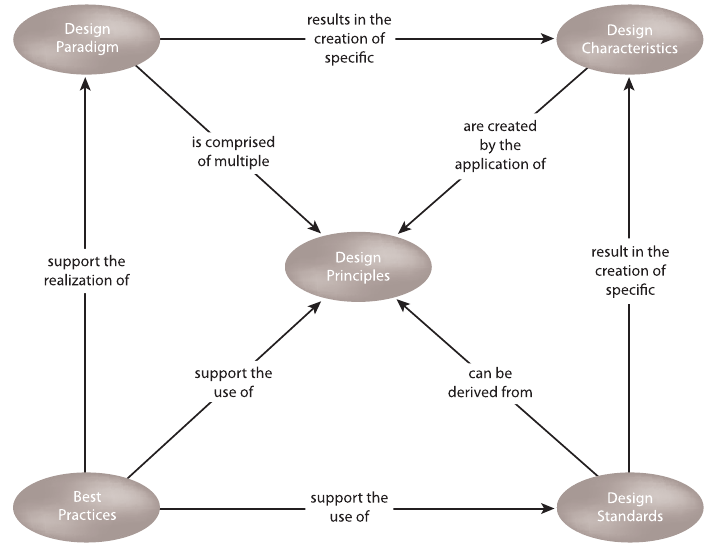
\includegraphics[width=11cm]{./imagenes/1.png}
    \caption{Ejemplo de uso del enlace exclusivo}
    \label{fig:uno}
  \end{center}
\end{figure}

La figura \ref{fig:dos} presenta cómo extiende o soporta un patrón de diseño el diseño lógico de la solución de software.

\begin{figure}[!htb]
  \begin{center}
    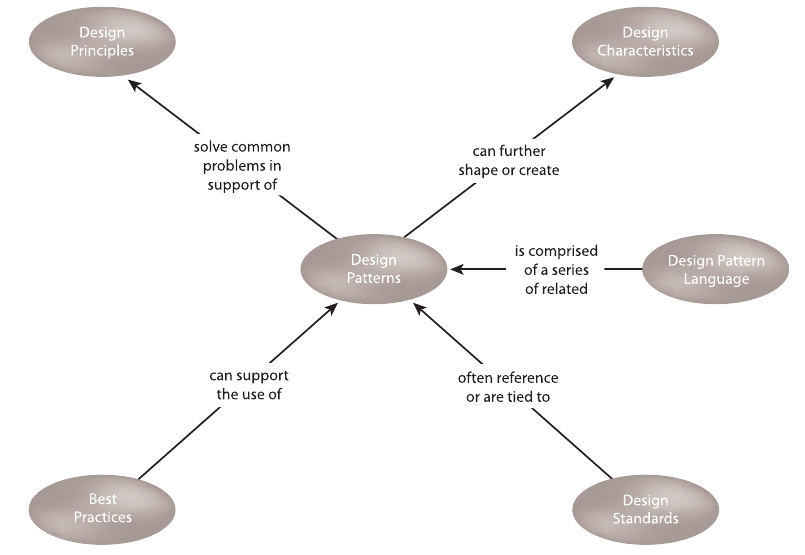
\includegraphics[width=11cm]{./imagenes/2.png}
    \caption{Ejemplo de uso del enlace exclusivo}
    \label{fig:dos}
  \end{center}
\end{figure}

La figura \ref{fig:tres} presenta los componentes que hacen que el diseño lógico de la solución sea acorde al paradigma escogido.

\begin{figure}[!htb]
  \begin{center}
    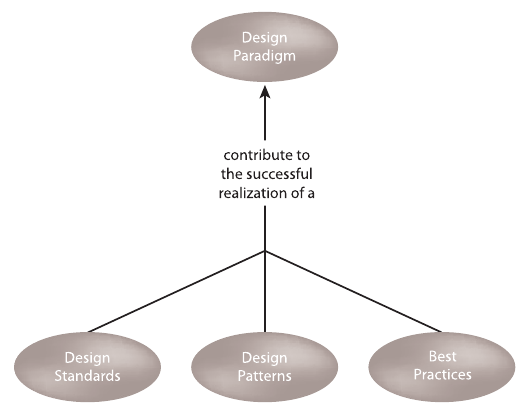
\includegraphics[width=11cm]{./imagenes/3.png}
    \caption{Ejemplo de uso del enlace exclusivo}
    \label{fig:tres}
  \end{center}
\end{figure}

\subsection{Computación orientada a servicios}

La computación orientada a servicios nace de la necesidad de desarrollar software sobre tecnologías distribuidas. Este tipo de computación tiene como finalidad la construcción de inventarios de servicios. La computación orientada a servicios está compuesta por la interacción de la orientación a servicios y la arquitectura orientada a servicios, formando patrones de diseño propios y estándares en cumplimiento de las características de diseño propias de la computación distribuida. Algunos de los conceptos clave llevados en la computación orientada a servicios son:

\begin{itemize}
  \item Arquitectura Orientada a Servicios (SOA - Service Oriented Architecture): Comprende el compendio de tecnologías, APIs, infraestructura y repositorios enmarcados en
el paradigma orientado a servicios y cuyo objetivo principal es el de trabajar sobre el "servicio" como el elemento más importante.

  \item Orientación a servicios: Es el paradigma manejado en la computación orientada a servicios en donde se acepta como unidad mínima y más importante el "servicio"

  \item Servicio: Es un software independiente físicamente el cual tiene asignado un contexto de funcionalidades y que puede ser utilizado por otros servicios por medio
del contrato del servicio (descripción del servicio en cuanto a funcionalidades, entradas requeridas y salidas). De acuerdo a su nivel de reuso, los servicios se dividen en 3 tipos y son:
  \item Servicios entidad: Modela los servicios que se deben ofrecer respecto de las entidades del negocio (ej. empleados y clientes). Tienen un nivel de reuso alto y están centrados en el negocio.
  \item Servicios tarea: Modela los servicios que deben cumplir tareas específicas del negocio (ej. generación de cortes de final de año). Tienen un nivel de reuso bajo. Estos servicios trabajan directamente con 1 o varios servicios entidad. Estos servicios están centrados en el negocio.
  \item Servicios utilidad: Modela servicios que no están centrados en el negocio. Son los servicios con mayor reuso.
La diferenciación entre tipos de servicio da lugar a la estructura en capas mostrada en la figura \ref{fig:cinco}

  \item Composición de servicios: Es la agregación de servicios de manera ordenada.

  \item Inventario de servicios: Es la agrupación de varios servicios según un criterio definido por la organización. Cada inventario de servicios tiene su propio estándar
de diseño e, inclusive, su propia configuración arquitectónica. El desarrollo de los inventarios de servicio es hecho a modo top-down, con la construcción de blueprints (planos).
\end{itemize}

\begin{figure}[!htb]
  \begin{center}
    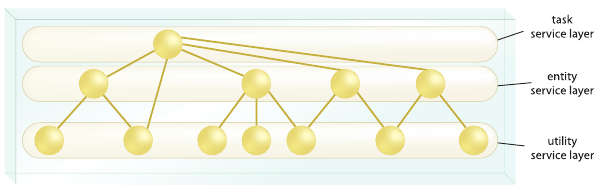
\includegraphics[width=11cm]{./imagenes/5.png}
    \caption{Ejemplo de uso del enlace exclusivo}
    \label{fig:cinco}
  \end{center}
\end{figure}

En la figura \ref{fig:cuatro} se muestra la interacción de los conceptos clave en la computación orientada a servicios.

\begin{figure}[!htb]
  \begin{center}
    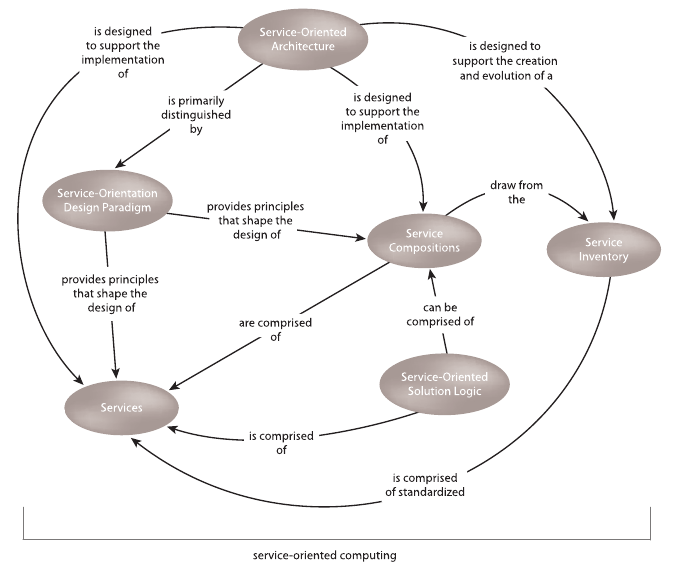
\includegraphics[width=11cm]{./imagenes/4.png}
    \caption{Ejemplo de uso del enlace exclusivo}
    \label{fig:cuatro}
  \end{center}
\end{figure}


\section{Scrum}

A continuación, se explican los diferentes roles y artefactos que existen en el marco de trabajo de Scrum.

\subsection{Equipo Scrum (Scrum Team)}

\subsubsection{Product Owner (dueño del producto)}

Es el responsable de gestionar el product backlog y el trabajo del equipo de desarrollo. Entre sus funciones se encuentran:
\begin{itemize}
		  \item Expresar los elementos del product backlog.
		  \item Ordenar de la mejor manera posible los elementos del product backlog para lograr el objetivo final.
		  \item Asegurarse de que el equipo de desarrollo entiende los items del product backlog.
		\end{itemize}
		
\subsubsection{Development Team (Equipo de desarrollo)}

Son los encargados de llevar a cabo el incremento al producto en cada iteración o sprint. El equipo de desarrollo es el encargado de organizar y gestionar su propio trabajo.

El equipo de desarrollo se caracteriza por:
	
\begin{itemize}
		  \item Es autoorganizado: Se le dice al equipo que debe hacer, pero el es libre de decidir como lo hace.
		  \item Son multifuncionales: Se tienen integrantes que manejan diferentes áreas de experticia para ayudar a realizar el incremento necesario.
		  \item No se reconocen los sub-equipos que se puedan formar, la responsabilidad de lo que se haga recae en e equipo de desarrollo como un todo.
		\end{itemize}

\subsubsection{Scrum Master}

Es el encargado de que se cumpla la teoría de scrum a lo largo de todo el proyecto. El Scrum Master ayuda a las personas externas al Equipo Scrum a entender qué interacciones con el Equipo Scrum pueden ser de ayuda y cuáles no \cite{scrum_guide}.

\textbf{Servicios que ofrece al Product Owner}
	
\begin{itemize}
		  \item Encontrar técnicas para gestionar la Lista de Producto de manera efectiva
		  \item Ayudar al Equipo Scrum a entender la necesidad de contar con elementos de Lista de Producto claros y concisos
		  \item Entender la planificación del producto en un entorno empírico
		  \item Asegurar que el Dueño de Producto conozca cómo ordenar la Lista de Producto para maximizar el valor
		  \item Entender y practicar la agilidad; y,
		  \item Facilitar los eventos de Scrum según se requiera o necesite.
\end{itemize}
		\cite{scrum_guide}

\textbf{Servicios que ofrece al Developement Team}
	
\begin{itemize}
		  \item Guiar al Equipo de Desarrollo en ser autoorganizado y multifuncional;
		  \item Ayudar al Equipo de Desarrollo a crear productos de alto valor;
		  \item Eliminar impedimentos para el progreso del Equipo de Desarrollo;
		  \item Facilitar los eventos de Scrum según se requiera o necesite; y,
		  \item Guiar al Equipo de Desarrollo en el entorno de organizaciones en las que Scrum aún no ha sido adoptado y entendido por completo.
\end{itemize}
		\cite{scrum_guide}

\textbf{Servicios que ofrece a la organización}
	
\begin{itemize}
		  \item Liderar y guiar a la organización en la adopción de Scrum;
		  \item Planificar las implementaciones de Scrum en la organización; 
		  \item Ayudar a los empleados e interesados a entender y llevar a cabo Scrum y el desarrollo empírico de producto;
		  \item Motivar cambios que incrementen la productividad del Equipo Scrum; y,
		  \item Trabajar con otros Scrum Masters para incrementar la efectividad de la aplicación de Scrum en la organización.
\end{itemize}
		\cite{scrum_guide}
		
\subsection{Eventos}

\subsubsection{Sprint}

El Sprint representa un espacio de tiempo, no mayor a un mes, en el que se trabaja para crear un incremento en el desarrollo del proyecto. Es conveniente que los sprint tengan una duración consistente a lo largo del proyecto, y un nuevo sprint inicia tan pronto el actual termina.

Cada sprint debe tener un objetivo definido (Sprint Goal), un plan flexible y concepto de ``terminado'' claro. 

\subsubsection{Sprint Planning Meeting (Reunión de Planificación de Sprint)}

Esta reunion se lleva a cabo al inicio de cada Sprint y no tiene una duración mayor a 8 horas. En esta reunión, que se lleva a cabo en presencia de todo el equipo scrum, se crea un plan para el sprint que inicia. En este plan se responden dos preguntas fundamentales, ¿Qué puede entregarse en el Incremento resultante del Sprint que comienza? y ¿Cómo se conseguirá hacer el trabajo necesario para entregar el Incremento?

\subsubsection{Daily Scrum (Scrum Diario)}

Esta reunion, que no debe durar mas de 15 minutos, se realiza a diario entre los miembros del development team. El objetivo de esta reunion es socializar lo que se hizo en las ultimas 24 horas y planear que hacer en las proximas 24 horas. Se evalua si se esta haciendo lo necesario para cumplir el sprint goal y, si es necesario, se puede adaptar o redefinir el trabajo del resto del sprint.

\subsubsection{Sprint Review (Revisión de Sprint)}

Al final de cada sprint se realiza esta reunion cuyo objetivo es el de socializar lo que se hizo en el presente sprint. En esta reunion se descuten cosas como qué fue bien durante el Sprint, qué problemas aparecieron y cómo fueron resueltos esos problemas. Al final de la revisión se debe generar un product backlog actualizado con los elementos que se proponen para el siguiente sprint. Esta reunion tiene una duracion no mayor a 4 horas.

\subsubsection{Sprint Retrospective (Retrospectiva de Sprint)}

Esta reunión es similar al sprint review, pero en lugar de tratar el Qué se hizo, se trata el Cómo se hizo. Al final de esta reunión se genera un plan para mejorar el desempeño del equipo de scrum para que los sprint posteriores sean de mayor provecho para el proyecto.

\subsection{Artefactos}

\subsubsection{Sprint Goal (Objetivo del Sprint)}

El sprint goal es una meta que se plantea al inicio de cada sprint que puede ser alcanzada mediante el incremento en el proyecto. Este sprint goal ``Proporciona una guía al Equipo de Desarrollo acerca de por qué está construyendo el incremento'' \cite{scrum_guide}. Es importante y necesario que el objetivo sea claro, coherente y sea entendido por todos los integrantes del equipo de scrum.

\subsubsection{Product Backlog (Lista de Producto)}

Esta lista representa todos los requisitos que tenga el proyecto o producto que son conocidos y entendidos en un momento determinado del desarrollo. Debido a la naturaleza cambiante y dinámica del entorno, la lista nunca está vacía. A medida que el producto evoluciona, la retroalimentación que se obtiene ayuda a completar la lista y a refinar el producto final.

\subsubsection{Sprint Backlog (Lista de Pendientes del Sprint)}

Esta lista esta compuesta por los diferentes items seleccionados del broduct backlog que van a ser tratados en cada sprint. Adicionalmente, se incluye un plan que ayude a conseguir el objetivo del sprint.
	
La Lista de Pendientes del Sprint es una predicción hecha por el Equipo de Desarrollo acerca de qué funcionalidad formará parte del próximo Incremento y del trabajo necesario para entregar esa funcionalidad en un Incremento \cite{scrum_guide}.


Una vez habiendo puesto en contexto el problema a resolver en los anteriores capítulos (en especial el capítulo \ref{chap:definicion_problema}), en este capítulo se encuentra una descripción un poco más concisa de los requerimientos funcionales encontrados por los autores y, también, los requerimientos no funcionales que serán tomados en cuenta a la hora de evaluar la calidad del prototipo del SNS desarrollado.

\section{Requerimientos funcionales}
La identificación de los requerimientos funcionales consignados en éste capítulo fue la base para realizar la arquitectura del software a implementar.

Se identificaron, en el análisis de requerimientos, 14 posibles módulos enunciados a continuación:

\begin{enumerate}
	\item \textbf{Gestión de usuarios*}: Módulo que controla características inherentes a todos los tipos de usuario de la red social en cuanto al manejo de su información personal y roles que cumplen
	\item \textbf{Gestión de deportes*}: Módulo por medio del cual se controla la información detallada de un deporte
	\item \textbf{Gestión de equipos}: Módulo que ayuda a la gestión de datos competentes a equipos deportivos
	\item \textbf{Gestión de torneos}: Módulo que suple las necesidades de un organizador de eventos cuando éste desea trabajar con la información de un torneo deportivo
	\item \textbf{Gestión de eventos deportivos*}: Módulo que brinda funcionalidades de gestión de eventos deportivos
	\item \textbf{Gestión de patrocinadores}: Módulo que brinda funcionalidades al patrocinador que lo use, para patrocinar y controlar patrocinios, así como para seguir actividad de posibles patrocinados.
	\item \textbf{Gestión de organizaciones}: Módulo que ofrece funciones de gestión de organizaciones
	\item \textbf{Gestión de self-expression}: Módulo que es utilizado para el manejo de contenido propio generado por un actor en la red social o un evento que uno o más actores manejen en la red social
	\item \textbf{Gestión del conocimiento}: Módulo que gestiona artículos/post relacionados con tips en campos de salud y deportivos en si
	\item \textbf{Gestión de geolocalización*}: Módulo que ayuda al control de todas las funcionalidades de geolocalización
	\item \textbf{Gestión de estadísticas}: Módulo que permite la generación y visualización de estadísticas diversas acerca de deportistas, organizaciones, ubicaciones o cualquier otro concepto que maneje estadísticas en el SNS
	\item \textbf{Gestión de entrenadores}: Módulo que permite la gestión de opcionalidades ofrecidas a entrenadores deportivos, tal como el seguimiento de entrenados o la asignación de planes deportivos a los mismos
	\item \textbf{Gestión de canales de difusión}: Módulo que refiere a todo lo relacionado con noticias deportivas
	\item \textbf{Gestión de grupos deportivos}:  Módulo de gestión de funcionalidades ofrecidas a grupos deportivos informales (diferentes a los equipos deportivos, caso especial de los grupos deportivos)
\end{enumerate}

Para el desarrollo del prototipo, los autores se concentran en los módulos marcados con * en la anterior lista. Para saber los criterios por los cuales se han escogido éstos módulos, el lector puede dirigirse a \ref{chap:alcances_limitaciones}.

La lista de requerimientos puede encontrarse en \ref{app:req_funcionales}.

\section{Requerimientos no funcionales}
Los requerimientos no funcionales explorados en detalle para el desarrollo del SNS deportivo y que son tenidos en cuenta se presentan a continuación con escenarios de calidad (reducidos; los escenarios completos se encuentran en \cite{anexos_tesis}), los cuales son descritos como los escenarios en los que se probará la calidad del software desarrollado.

\subsubsection{QiU}

En esta sección se da una versión simplificada del análisis de escenarios de calidad correspondientes a las áreas de usabilidad y UX.

\begin{itemize}
	\item \textbf{Escenario de calidad 1}: Busca que el usuario pueda realizar todas las tareas que desea realizar con el SNS
	\item \textbf{Escenario de calidad 2}: Busca que las funcionalidades ofrecidas por el SNS se ejecuten en un tiempo corto
	\item \textbf{Escenario de calidad 3}: Busca que el nivel de conformidad con la interfaz de usuario (UX) sea marcado
	\item \textbf{Escenario de calidad 4}: Busca que el usuario aprenda a utilizar las principales funcionalidades del SNS en poco tiempo
	\item \textbf{Escenario de calidad 5}: Busca hacer legible cada mensaje de error que aparezca cada vez que se produzca uno en el SNS
	\item \textbf{Escenario de calidad 6}: Busca hacer conciente al usuario de los diferentes roles manejados a través de la red social
	\item \textbf{Escenario de calidad 7}: Busca que el usuario conozca todas las funcionalidades ofrecidas por el SNS
	\item \textbf{Escenario de calidad 8}: Busca que el usuario sea efectivo a la hora de utilizar cada funcionalidad
\end{itemize}

\subsubsection{Reusabilidad}

Para el desarrollo de escenarios de calidad en cuanto a reusabilidad se refiere, se utilizaron apartes de \cite{soa_principles} para definirlos. A continuación se exponen los escenarios de calidad resumidos.

\begin{itemize}
	\item \textbf{Escenario de calidad 1}: Busca que el software cumpla con la reusabilidad táctica
	\item \textbf{Escenario de calidad 2}: Busca dar a los servicios hechos en la red social, en su mayoría, un carácter agnóstico
	\item \textbf{Escenario de calidad 3}: Busca la estandarización del nombramiento de las diferentes partes de los contratos de servicio a crear
\end{itemize}

\subsubsection{Mantenibilidad}

A continuación se exponen escenarios de calidad resumidos relacionados a la mantenibilidad, tomando como base tanto el paradigma orientado a servicios como elementos del estandar ISO/IEC 9126.

\begin{itemize}
	\item \textbf{Escenario de calidad 1}: Busca mayor adaptación del software a capacidades nuevas
	\item \textbf{Escenario de calidad 2}: Busca disminuir la cantidad de lógica envuelta por un servicio
	\item \textbf{Escenario de calidad 3}: Busca que los servicios tengan una complejidad tan manejable como sea posible
\end{itemize}

\subsubsection{Interoperabilidad}

En \cite{soa_principles}, se hace referencia a la interoperabilidad como un componente transversal a todo principio, patrón y demás concepto manejado en el paradigma orientado a servicios. A continuación se describe el escenario de calidad resumido estipulado por los autores.

\begin{itemize}
	\item \textbf{Escenario de calidad 1}: Busca la adopción de una política estricta de estandarización al momento del desarrollo de los contratos de servicio
\end{itemize}

\subsubsection{Seguridad}

Se tuvieron en cuenta los principios de seguridad expresados en \cite{security_ws}. A continuación se enuncian los escenarios de calidad resumidos estipulados por el lado de la seguridad.

\begin{itemize}
	\item \textbf{Escenario de calidad 1}: Busca aplicar el concepto de ''Fail Securely''
	\item \textbf{Escenario de calidad 2}: Busca deshabilitar toda funcionalidad no terminada y accesos a ellas
	\item \textbf{Escenario de calidad 3}: Busca establecer un sistema de autenticación-autorización
	\item \textbf{Escenario de calidad 4}: Busca la encripción de mensajes pasados entre servicios
\end{itemize}

\subsubsection{Rendimiento}

Para el rendimiento, \cite{time_response}, se tuvo en cuenta una sola medida: Las funcionalidades que no dependan de la carga o descarga de una cantidad de información grande (ej. videos e imágenes) no deberán tardar más de 5 segundos.

\section{Archimate 2.0}

Según  \cite{archimate2}, archimate es un lenguaje estandar utilizado por los arquitectos de software para modelar las necesidades de cada \textit{stakeholder}, dividiendo el contexto en el que se desenvuelve el software a desarrollar en tres capas: capa de negocio, capa de aplicación y capa de tecnología.

\subsection{Capas de archimate}

A continuación serán descritas las tres capas definidas en el estandar archimate.

\subsubsection{Capa de negocio}

Esta capa envuelve todos los conceptos relacionados con la organización sobre la cual se aplicará el software a desarrollar, esto es, los roles, los servicios ofrecidos, los procesos, los productos y demás conceptos aplicados sobre su estructura y dinámica. Los artefactos de esta capa utilizados en el proyecto se enuncian en el cuadro \ref{tab:artefactos_capa_negocio}.

 \begin{center}
 
 	\textbf{Fuente:} \cite{archimate2}
 	
	\begin{longtable}{|p{4cm}|p{6cm}|c|}
	\caption{Artefactos de la capa de negocio \label{tab:artefactos_capa_negocio}} \\
	\hline
    \textbf{Artefacto} & 
    \textbf{Descripción} & 
    \textbf{Notación} \\ 
    \hline
	\endfirsthead
    \hline
    \textbf{Artefacto} & 
    \textbf{Descripción} & 
    \textbf{Notación} \\ 
    \hline
	\endhead
    \hline
	\endfoot
	\hline
	\endlastfoot
    \hline
    \textit{Actor de negocio (Business actor)} & 
    Ente (persona) organizacional quien cumple tareas en la organización &  
    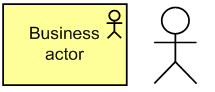
\includegraphics[width=1.5cm]{./imagenes/Archimate/businessactor.png}\\
	\hline
	\textit{Colaboración de negocio (Business collaboration)} & 
    Rol que surge de la combinación de dos o más roles &  
    \includegraphics[width=1.5cm]{./imagenes/Archimate/businesscollaboration.png}\\
	\hline    
    \textit{Rol de negocio (Business role)} & 
    Es un conjunto de responsabilidades que tiene asignado un actor. Dicho conjunto está definido por un solo concepto (nombre) &  
    \includegraphics[width=1.5cm]{./imagenes/Archimate/businessrole.png}\\
    \hline
    \textit{Proceso de negocio (Business process)} & 
    Agrupa comportamientos que se ejecutan como una serie de pasos &  
    \includegraphics[width=1.5cm]{./imagenes/Archimate/businessprocess.png}\\
	\hline
	\textit{Función de negocio (Business function)} & 
    Agrupa comportamientos que requieren una serie de competencias o recursos de negocio &  
    \includegraphics[width=1.5cm]{./imagenes/Archimate/businessfunction.png}\\
	\hline
	\textit{Interacción de negocio (Business interaction)} & 
    Comportamientos realizados por colaboraciones de negocio &  
    \includegraphics[width=1.5cm]{./imagenes/Archimate/businessinteraction.png}\\
	\hline
	\textit{Evento de negocio (Business event)} & 
    Hecho que dispara un comportamiento (o grupo de comportamientos) en la organización &  
    \includegraphics[width=1.5cm]{./imagenes/Archimate/businessevent.png}\\
	\hline
	\textit{Servicio de negocio (Business service)} & 
    Servicio que cumple una necesidad del usuario &  
    \includegraphics[width=1.5cm]{./imagenes/Archimate/businessservice.png}\\
	\hline
	\textit{Producto (Product)} & 
    Agrupación de servicios que, definidos por un contrato, serán compartidos a clientes (tanto roles dentro de la organización como para clientes externos) &  
    \includegraphics[width=1.5cm]{./imagenes/Archimate/businessproduct.png}\\
	\hline
  \end{longtable}
\end{center}

\subsubsection{Capa de aplicación} 

Esta capa cubre los conceptos relacionados con el modelamiento del sistema de información que soporta el negocio (la organización), previamente modelado en la capa de negocio. Los artefactos de esta capa utilizados en el proyecto se enuncian en el cuadro \ref{tab:artefactos_capa_aplicacion}.

\begin{table}
  \caption{Artefactos de la capa de aplicación}
  \label{tab:artefactos_capa_aplicacion}

  \begin{center}
  
  \textbf{Fuente:} \cite{archimate2}
  
  \resizebox{15cm}{!}{
  \begin{tabular}{|L{3cm}|L{6cm}|c|}
    \hline
    \textbf{Artefacto} & \textbf{Descripción} & \textbf{Notación} \\ 
    \hline
    \textit{Componente de aplicación (Application component)} & 
    Unidad de software &  
    \includegraphics[width=1.5cm]{./imagenes/Archimate/applicationcomponent.png}\\
	\hline
	\textit{Colaboración de aplicación (Application collaboration)} & 
    Colaboración entre dos o más componentes de aplicación para realizar una tarea que necesita de cada uno de ellos &  
    \includegraphics[width=1.5cm]{./imagenes/Archimate/applicationcollaboration.png}\\
	\hline    
    \textit{Función de aplicación (Application function)} & 
    Agrupa comportamientos que pueden ser automatizados por un componente de aplicación &  
    \includegraphics[width=1.5cm]{./imagenes/Archimate/applicationfunction.png}\\
    \hline
    \textit{Interacción de aplicación (Application interaction)} & 
    Agrupa comportamientos que pueden ser automatizados por una colaboración de aplicación &  
    \includegraphics[width=1.5cm]{./imagenes/Archimate/applicationinteraction.png}\\
	\hline
	\textit{Servicio de aplicación (Application service)} & 
    Un servicio que expone las funcionalidades automatizadas ofrecidas &  
    \includegraphics[width=1.5cm]{./imagenes/Archimate/applicationservice.png}\\
	\hline
  \end{tabular}
  }
    \end{center}
\end{table}

\subsubsection{Capa de tecnología}

Capa que modela el posicionamiento físico del software a utilizar, así como también los requerimientos que este tiene para su funcionamiento a nivel físico (servidores, redes, nodos, etc.). Los artefactos de esta capa utilizados en el proyecto se enuncian en el cuadro \ref{tab:artefactos_capa_tecnologia}.


\begin{table}
  \caption{Artefactos de la capa de tecnología}
  \label{tab:artefactos_capa_tecnologia}

  \begin{center}
  
  \textbf{Fuente:} \cite{archimate2}
  
  \resizebox{15cm}{!}{
  \begin{tabular}{|L{3cm}|L{6cm}|c|}
    \hline
    \textbf{Artefacto} & \textbf{Descripción} & \textbf{Notación} \\ 
    \hline
    \textit{Nodo (Node)} & 
    Recurso computacional que agrupa artefactos almacenables o desplegables para ser ejecutados &  
    \includegraphics[width=1.5cm]{./imagenes/Archimate/technologynode.png}\\
	\hline
	\textit{Dispositivo (Device)} & 
    Hardware que contiene elementos software para ser ejecutados &  
    \includegraphics[width=1.5cm]{./imagenes/Archimate/technologydevice.png}\\
	\hline    
    \textit{Red (Network)} & 
    Medio de comunicación entre dos o más nodos o dispositivos &  
    \includegraphics[width=1.5cm]{./imagenes/Archimate/technologynetwork.png}\\
    \hline
    \textit{Sistema de software (System software)} & 
    Software sobre el cual se realizan (o representan) los artefactos (componentes de aplicación) desplegables &  
    \includegraphics[width=1.5cm]{./imagenes/Archimate/technologyswsystem.png}\\
	\hline
	\textit{Servicio de infraestructura (Infraestructure service)} & 
    Servicios que agrupan funcionalidades prestadas por nodos &  
    \includegraphics[width=1.5cm]{./imagenes/Archimate/technologyservice.png}\\
	\hline
  \end{tabular}
  }
    \end{center}
\end{table}

\subsection{Relaciones}

Las relaciones, en archimate, son aquellas conexiones existentes entre dos artefactos. Hay tres tipos de relaciones en archimate: relaciones estructurales, relaciones dinámicas y otras que no caben en las dos últimas.

\begin{itemize}

\item \textbf{Relaciones estructurales}: Estas relaciones modelan la coherencia estructural generada por la unión estructural de todos los artefactos de la arquitectura. En el cuadro \ref{tab:relaciones_estructurales} se hace un sumario de las relaciones estructurales utilizadas para unir los artefactos utilizados en el presente proyecto:

\begin{table}
  \caption{Relaciones estructurales}
  \label{tab:relaciones_estructurales}

  \begin{center}
  
  \textbf{Fuente:} \cite{archimate2}
  
  \resizebox{15cm}{!}{
  \begin{tabular}{|L{3cm}|L{7cm}|c|}
    \hline
    \textbf{Relación} & \textbf{Descripción} & \textbf{Notación} \\ 
    \hline
    \textit{Asociación (Association)} & 
    Cumple la función de asociar dos artefactos que no tienen una relación más específica &  
    \includegraphics[width=1cm]{./imagenes/Archimate/relassociation.png}\\
	\hline
	\textit{Usado por (Used by)} & 
    Modela el acceso a servicios o interfaces. El acceso a interfaces solo puede ser realizado por artefactos estructurales y a los servicios solo los artefactos comportamentales &  
    \includegraphics[width=1cm]{./imagenes/Archimate/relusedby.png}\\
	\hline    
    \textit{Realización (Realization)} & 
    Une un artefacto abstracto con otro más concreto que lo realiza &  
    \includegraphics[width=1cm]{./imagenes/Archimate/relrealization.png}\\
    \hline
    \textit{Asignación (Assignment)} & 
    Une artefactos con aquellos que, por obligación, deben utilizar otros (por ejemplo, un rol con una función de negocio) &  
    \includegraphics[width=1cm]{./imagenes/Archimate/relassignment.png}\\
	\hline
	\textit{Agregación (Aggregation)} & 
    Es la composición de un artefacto por otros. Esta composición no es destructiva, es decir, si el artefacto que es compuesto deja de existir, los otros seguirán existiendo &  
    \includegraphics[width=1cm]{./imagenes/Archimate/relaggregation.png}\\
	\hline
	\textit{Composición (Composition)} & 
    Es la composición de un artefacto por otros. Esta composición es destructiva, es decir, si el artefacto que es compuesto deja de existir, los otros también &  
    \includegraphics[width=1cm]{./imagenes/Archimate/relcomposition.png}\\
	\hline
  \end{tabular}
  }
    \end{center}
\end{table}

\item \textbf{Relaciones dinámicas}: Esta relación expresa una unión temporal entre dos artefactos donde, posiblemente, uno de los artefactos use a otro para cumplir un fin específico.En el cuadro \ref{tab:relaciones_dinamicas} se hace un sumario de las relaciones dinámicas utilizadas para unir los artefactos utilizados en el presente proyecto.

\begin{table}
  \caption{Relaciones dinámicas}
  \label{tab:relaciones_dinamicas}

  \begin{center}
  
  \textbf{Fuente:} \cite{archimate2}
  
  \resizebox{15cm}{!}{
  \begin{tabular}{|L{3cm}|L{7cm}|c|}
    \hline
    \textbf{Relación} & \textbf{Descripción} & \textbf{Notación} \\ 
    \hline
    \textit{Flujo (Flow)} & 
    Describe intercambios de información entre artefactos comportamentales &  
    \includegraphics[width=1.5cm]{./imagenes/Archimate/relflow.png} 
    \\
	\hline
	\textit{Disparador (Triggering)} & 
    Describe la relación temporal o factual entre 2 artefactos comportamentales &  
    \includegraphics[width=1.5cm]{./imagenes/Archimate/reltriggering.png}
    \\
	\hline
  \end{tabular}
  }
    \end{center}
\end{table}

\item \textbf{Otras relaciones}: En el cuadro \ref{tab:otras_relaciones} se hace un sumario de las relaciones que no pueden ser incluidas en las dinámicas o en las estructurales y que son utilizadas para unir los artefactos utilizados en el presente proyecto.

\begin{table}
  \caption{Otras relaciones}
  \label{tab:otras_relaciones}

  \begin{center}
  
  \textbf{Fuente:} \cite{archimate2}
  
  \resizebox{15cm}{!}{
  \begin{tabular}{|L{3cm}|L{7cm}|c|}
    \hline
    \textbf{Relación} & \textbf{Descripción} & \textbf{Notación} \\ 
    \hline
    \textit{Unión (Junction)} & 
    Cumple la función de asociar dos artefactos que no tienen una relación más específica &  
    \includegraphics[width=1cm]{./imagenes/Archimate/reljunction.png}\\
	\hline
	\textit{Especialización (Specialization)} & 
    Indica la especialización de un artefacto tomando otro como referencia &  
    \includegraphics[width=1cm]{./imagenes/Archimate/relspecialization.png}\\
	\hline
  \end{tabular}
  }
    \end{center}
\end{table}

\end{itemize}

\subsection{Vistas archimate}

Debido a la existencia de diferentes stakeholders en el desarrollo de software, se hace necesario mostrar aquella parte de la arquitectura que cierto stakeholder necesita para tener una vista entera del negocio, el sistema de información o la infraestructura, o bien una combinación de ellos.

Archimate utiliza el concepto de “vistas” como la segmentación de la arquitectura en vistas que conciernen al stakeholder que quiera echar un vistaso a la arquitectura, escondiendo detalles de la arquitectura que no le interesan a este.

En los cuadros \ref{tab:introductory_viewpoint} a \ref{tab:infrastructure_viewpoint} se pueden ver las vistas utilizadas, con su descripción y su metamodelo.

\begin{table}
  \caption{Punto de vista introductorio}
  \label{tab:introductory_viewpoint}

  \begin{center}
  
  \textbf{Fuente:} \cite{archimate2}
  
  \resizebox{15cm}{!}{
  \begin{tabular}{|L{4cm}|L{11cm}|}
    \hline
    \textbf{Punto de vista} & 
    Punto de vista introductorio (introductory viewpoint) \\ 
    \hline
    \textbf{Stakeholders} & 
    Arquitectos empresariales y gerentes generales \\ 
    \hline
    \textbf{Concerns} & 
    Da un panorama de los cambios, representaciones o adiciones del o a la organización. Ayuda a la toma de decisiones \\ 
    \hline
    \textbf{Propósito} & 
    Diseñar, decidir e informar \\ 
    \hline
    \textbf{Capas} & 
    Negocio, aplicación e infraestructura \\ 
    \hline
    \textbf{Metamodelo} &
    \includegraphics[width=7cm]{./imagenes/Archimate/introductoryviewpoint.png}\\
	\hline
  \end{tabular}
  }
    \end{center}
\end{table}

\begin{table}
  \caption{Punto de vista en capas}
  \label{tab:layered_viewpoint}

  \begin{center}
  
  \textbf{Fuente:} \cite{archimate2}
  
  \resizebox{15cm}{!}{
  \begin{tabular}{|L{4cm}|L{11cm}|}
    \hline
    \textbf{Punto de vista} & 
    Punto de vista en capas (layered viewpoint) \\ 
    \hline
    \textbf{Stakeholders} & 
    Arquitectos de dominio, infraestructura, procesos, aplicación y negocio \\ 
    \hline
    \textbf{Concerns} & 
    Impacto del cambio, flexibilidad, reducción de la complejidad y consistencia \\ 
    \hline
    \textbf{Propósito} & 
    Diseñar, decidir e informar \\ 
    \hline
    \textbf{Capas} & 
    Negocio, aplicación e infraestructura \\ 
    \hline
    \textbf{Metamodelo} &
    Se usan los artefactos y relaciones de todas las capas, según se considere pertinente\\
	\hline
  \end{tabular}
  }
    \end{center}
\end{table}

\begin{table}
  \caption{Punto de vista de función}
  \label{tab:business_function_viewpoint}

  \begin{center}
  
  \textbf{Fuente:} \cite{archimate2}
  
  \resizebox{15cm}{!}{
  \begin{tabular}{|L{4cm}|L{11cm}|}
    \hline
    \textbf{Punto de vista} & 
    Punto de vista de función (business function viewpoint) \\ 
    \hline
    \textbf{Stakeholders} & 
    Organización, arquitectos de proceso y de dominio \\ 
    \hline
    \textbf{Concerns} & 
    Identificación de competencias, identificación de actividades principales y reducción de complejidad \\ 
    \hline
    \textbf{Propósito} & 
    Diseño \\ 
    \hline
    \textbf{Capas} & 
    Negocio \\ 
    \hline
    \textbf{Metamodelo} &
    \includegraphics[width=7cm]{./imagenes/Archimate/businessfunctionviewpoint.png}\\
	\hline
  \end{tabular}
  }
    \end{center}
\end{table}

\begin{table}
  \caption{Punto de vista de proceso}
  \label{tab:business_process_viewpoint}

  \begin{center}
  
  \textbf{Fuente:} \cite{archimate2}
  
  \resizebox{15cm}{!}{
  \begin{tabular}{|L{4cm}|L{11cm}|}
    \hline
    \textbf{Punto de vista} & 
    Punto de vista de proceso (business process viewpoint) \\ 
    \hline
    \textbf{Stakeholders} & 
    Gerentes operacionales, aquitectos de dominio y de proceso \\ 
    \hline
    \textbf{Concerns} & 
    Estructura del proceso de negocio, consistencia y completitud así como también responsabilidades \\ 
    \hline
    \textbf{Propósito} & 
    Diseño \\ 
    \hline
    \textbf{Capas} & 
    Negocio y aplicación \\ 
    \hline
    \textbf{Metamodelo} &
    \includegraphics[width=7cm]{./imagenes/Archimate/businessprocessviewpoint.png}\\
	\hline
  \end{tabular}
  }
    \end{center}
\end{table}

\begin{table}
  \caption{Punto de vista de uso de aplicación}
  \label{tab:application_usage_viewpoint}

  \begin{center}
  
  \textbf{Fuente:} \cite{archimate2}
  
  \resizebox{15cm}{!}{
  \begin{tabular}{|L{4cm}|L{11cm}|}
    \hline
    \textbf{Punto de vista} & 
    Punto de vista de uso de aplicación (Application usage viewpoint) \\ 
    \hline
    \textbf{Stakeholders} & 
    Arquitectos de proceso, arquitectos de negocio, arquitectos de aplicación y gerentes operacionales \\ 
    \hline
    \textbf{Concerns} & 
    Competencia y completitud, reducción de la complejidad \\ 
    \hline
    \textbf{Propósito} & 
    Diseño y decisión \\ 
    \hline
    \textbf{Capas} & 
    Negocio y aplicación \\ 
    \hline
    \textbf{Metamodelo} &
    \includegraphics[width=7cm]{./imagenes/Archimate/applicationusageviewpoint.png}\\
	\hline
  \end{tabular}
  }
    \end{center}
\end{table}

\begin{table}
  \caption{Punto de vista de producto}
  \label{tab:product_viewpoint}

  \begin{center}
  
  \textbf{Fuente:} \cite{archimate2}
  
  \resizebox{15cm}{!}{
  \begin{tabular}{|L{4cm}|L{11cm}|}
    \hline
    \textbf{Punto de vista} & 
    Punto de vista de producto (Product viewpoint) \\ 
    \hline
    \textbf{Stakeholders} & 
    Desarrolladores de producto, gerentes de producto y de proceso, también los arquitectos de dominio \\ 
    \hline
    \textbf{Concerns} & 
    Desarrollo de producto y muestra del valor ofrecido por los productos de la organización \\ 
    \hline
    \textbf{Propósito} & 
    Diseño y decisión \\ 
    \hline
    \textbf{Capas} & 
    Negocio y aplicación \\ 
    \hline
    \textbf{Metamodelo} &
    \includegraphics[width=7cm]{./imagenes/Archimate/productviewpoint.png}
    \\
	\hline
  \end{tabular}
  }
    \end{center}
\end{table}

\begin{table}
  \caption{Punto de vista de producto}
  \label{tab:infrastructure_viewpoint}

  \begin{center}
  
  \textbf{Fuente:} \cite{archimate2}
  
  \resizebox{15cm}{!}{
  \begin{tabular}{|L{4cm}|L{11cm}|}
    \hline
    \textbf{Punto de vista} & 
    Punto de vista de infraestructura (Infrastructure viewpoint) \\ 
    \hline
    \textbf{Stakeholders} & 
    Arquitectos de infraestructura, gerente de operaciones \\ 
    \hline
    \textbf{Concerns} & 
    Estabilidad, seguridad, dependencias y costos de infraestructura \\ 
    \hline
    \textbf{Propósito} & 
    Diseño \\ 
    \hline
    \textbf{Capas} & 
    Tecnología \\ 
    \hline
    \textbf{Metamodelo} &
    \includegraphics[width=7cm]{./imagenes/Archimate/infrastructureviewpoint.png}
    \\
	\hline
  \end{tabular}
  }
    \end{center}
\end{table}

\section{Estado del arte} \label{cap:estado_arte}

Se hizo una búsqueda de redes sociales basadas en deporte que existen actualmente en la red. Una vez encontradas, se eligieron exactamente 16 SNS deportivas que ofrecían, en conjunto, las funcionalidades que se observaban en las demás redes sociales que no fueron escogidas (Cuadros \ref{tab:comparacion_redes_1} a \ref{tab:comparacion_redes_5}). Luego de la elección de la muestra de SNS, se reunieron aspectos de cada una hasta formar un grueso de sus funcionalidades y se realizó un cuadro de Funcionalidades vs SNS en donde se expresa con detalle cómo se presenta cada funcionalidad con respecto a cada SNS (en caso de no haber una conexión funcionalidad – SNS, entonces la casilla se dejó en blanco). En los cuadros \ref{tab:comparacion_redes_1} a \ref{tab:comparacion_redes_5} se da evidencia del análisis Funcionalidad vs SNS realizado.

Cada una de las funcionalidades que fueron descubiertas en otros SNS deportivos ya creados son el primer paso, pues, para conocer las necesidades de los usuarios de los SNS deportivos. El análisis de estos SNS será, entonces, el punto de partida para definir los requerimientos funcionales del SNS que plantearemos desde el punto de vista funcional.

\begin{landscape}
  
\begin{table}
  \caption{Comparacion de redes, parte 1}
  \label{tab:comparacion_redes_1}

  \begin{center}
  
  \textbf{Fuente:} Autores.
  
  \resizebox{20cm}{!}{
  \begin{tabular}{|p{5cm}|llll|}
    \hline
    Fun\textbackslash Red social & \multicolumn{1}{c}{Sportfactor} & \multicolumn{1}{c}{Deportesreunidos} & \multicolumn{1}{c}{Mybestplay} & \multicolumn{1}{c|}{Subetudeporte} \\ 
    \hline
    Gestión de foros & \multicolumn{1}{c}{} & \multicolumn{1}{c}{Si} & \multicolumn{1}{c}{} & \multicolumn{1}{c|}{Si} \\ 
    \hline
    Gestión de encuentros deportivos & \multicolumn{1}{c}{} & \multicolumn{1}{c}{- Organización de eventos} & \multicolumn{1}{c}{} & \multicolumn{1}{c|}{} \\ 
     & \multicolumn{1}{c}{} & \multicolumn{1}{c}{-Encuentros deportivos informales} & \multicolumn{1}{c}{} & \multicolumn{1}{c|}{} \\ 
     & \multicolumn{1}{c}{} & \multicolumn{1}{c}{} & \multicolumn{1}{c}{} & \multicolumn{1}{c|}{} \\ 
    \hline
    Creación de grupos & \multicolumn{1}{c}{} & \multicolumn{1}{c}{Si} & \multicolumn{1}{c}{} & \multicolumn{1}{c|}{} \\ 
    \hline
    Manejo de torneos & \multicolumn{1}{c}{} & \multicolumn{1}{c}{- Organización y difusión} & \multicolumn{1}{c}{} & \multicolumn{1}{c|}{} \\ 
    \hline
    Difusión info. Deportiva & \multicolumn{1}{c}{-RSS de noticias} & \multicolumn{1}{c}{- Blog propio} & \multicolumn{1}{c}{-Difusión de eventos} & \multicolumn{1}{c|}{- Gestión de blogs} \\ 
     & \multicolumn{1}{c}{} & \multicolumn{1}{c}{} & \multicolumn{1}{c}{-Blog propio} & \multicolumn{1}{c|}{} \\ 
    \hline
    Serv. self-expression & \multicolumn{1}{c}{} & \multicolumn{1}{c}{-Difusión de multimedia} & \multicolumn{1}{c}{-Difusión de multimedia } & \multicolumn{1}{c|}{-Difusión de multimedia} \\ 
     & \multicolumn{1}{c}{} & \multicolumn{1}{c}{} & \multicolumn{1}{c}{} & \multicolumn{1}{c|}{} \\ 
    \hline
    Sistema estadístico & \multicolumn{1}{c}{-Medición de avance en} & \multicolumn{1}{c}{- Sistemas de estadísticas para cada servicio} & \multicolumn{1}{c}{} & \multicolumn{1}{c|}{} \\ 
     & \multicolumn{1}{c}{ estadísticas del deporte practicado} & \multicolumn{1}{c}{} & \multicolumn{1}{c}{} & \multicolumn{1}{c|}{} \\ 
    \hline
    Gestión de transversales & \multicolumn{1}{c}{-Trainner personales} & \multicolumn{1}{c}{} & \multicolumn{1}{c}{} & \multicolumn{1}{c|}{} \\ 
     & \multicolumn{1}{c}{-Guías de nutrición} & \multicolumn{1}{c}{} & \multicolumn{1}{c}{} & \multicolumn{1}{c|}{} \\ 
     & \multicolumn{1}{c}{- Catalogo de lesiones y fisioterapia} & \multicolumn{1}{c}{} & \multicolumn{1}{c}{} & \multicolumn{1}{c|}{} \\ 
    \hline
    Servicios deportivos & \multicolumn{1}{c}{-Guía deportiva (shops, restaurantes, etc.)} & \multicolumn{1}{c}{} & \multicolumn{1}{c}{} & \multicolumn{1}{c|}{} \\ 
     & \multicolumn{1}{c}{} & \multicolumn{1}{c}{} & \multicolumn{1}{c}{} & \multicolumn{1}{c|}{} \\ 
    \hline
    Soporte multi-deporte & \multicolumn{1}{c}{Si} & \multicolumn{1}{c}{Si} & \multicolumn{1}{c}{Solo deportes en equipo} & \multicolumn{1}{c|}{Si} \\ 
    \hline
    Gestión de tipos de usu. & \multicolumn{1}{c}{} & \multicolumn{1}{c}{- Equipos } & \multicolumn{1}{c}{Si} & \multicolumn{1}{c|}{} \\ 
     & \multicolumn{1}{c}{} & \multicolumn{1}{c}{- Clubes} & \multicolumn{1}{c}{} & \multicolumn{1}{c|}{} \\ 
     & \multicolumn{1}{c}{} & \multicolumn{1}{c}{-Centros deportivos} & \multicolumn{1}{c}{} & \multicolumn{1}{c|}{} \\ 
    \hline
    Gestión de sponsors & \multicolumn{1}{c}{} & \multicolumn{1}{c}{} & \multicolumn{1}{c}{Si} & \multicolumn{1}{c|}{} \\ 
    \hline
    Gestión del conocimiento & \multicolumn{1}{c}{} & \multicolumn{1}{c}{} & \multicolumn{1}{c}{} & \multicolumn{1}{c|}{} \\ 
    \hline
    Gestión de geolocaliza. & \multicolumn{1}{c}{} & \multicolumn{1}{c}{} & \multicolumn{1}{c}{} & \multicolumn{1}{c|}{} \\ 
     & \multicolumn{1}{c}{} & \multicolumn{1}{c}{} & \multicolumn{1}{c}{} & \multicolumn{1}{c|}{} \\ 
    \hline
    Soporte móvil & \multicolumn{1}{c}{} & \multicolumn{1}{c}{} & \multicolumn{1}{c}{} & \multicolumn{1}{c|}{} \\ 
     & \multicolumn{1}{c}{} & \multicolumn{1}{c}{} & \multicolumn{1}{c}{} & \multicolumn{1}{c|}{} \\ 
    \hline
    Conexión con otros SNS & \multicolumn{1}{c}{} & \multicolumn{1}{c}{} & \multicolumn{1}{c}{} & \multicolumn{1}{c|}{} \\ 
     & \multicolumn{1}{c}{} & \multicolumn{1}{c}{} & \multicolumn{1}{c}{} & \multicolumn{1}{c|}{} \\ 
    \hline
  \end{tabular}
  }
    \end{center}
\end{table}
  
  \newpage
  
  \begin{table}
  \caption{Comparacion de redes, parte 2}
  \label{tab:comparacion_redes_2}

  \begin{center}
  
  \textbf{Fuente:} Autores.
  
  \resizebox{20cm}{!}{
    \begin{tabular}{|p{4cm}|p{9cm}p{7cm}p{7cm}|}
\hline
Fun\textbackslash Red social & Sporttia & Amatteur & Fitivity  \\ 
\hline
Gestión de foros &  &  &  \\ 
\hline
Gestión de encuentros deportivos & - Organización de eventos en centros deportivos & - Publicación o búsqueda de eventos deportivos & -Basado en geolocalización \\ 
 & - Gestión de jugadores &  &  \\ 
 & -Gestión de características del partido &  &  \\ 
\hline
Creación de grupos &  &  &  \\ 
\hline
Manejo de torneos &  &  &  \\ 
\hline
Difusión info. Deportiva &  &  &  \\ 
 &  &  &  \\ 
\hline
Serv. self-expression &  & -Difusión de multimedia &  \\ 
 &  &  &  \\ 
\hline
Sistema estadístico &  &  &  \\ 
 &  &  &  \\ 
\hline
Gestión de transversales &  &  &  \\ 
 &  &  &  \\ 
 &  &  &  \\ 
\hline
Servicios deportivos & -Alquiler de centros deportivos & - Servicios de compra y venta de artículos deportivos &  \\ 
 &  &  &  \\ 
\hline
Soporte multi-deporte & Si & Si & Si \\ 
\hline
Gestión de tipos de usu. & -Deportista -Centro deportivo & -Deportista  &  \\ 
 &  & -Equipo &  \\ 
 &  &  -Organización &  \\ 
\hline
Gestión de sponsors &  & -Promoción como deportista, equipo u organización &  \\ 
\hline
Gestión del conocimiento & - Clases virtuales &  &  \\ 
\hline
Gestión de geolocaliza. &  & Si & Si \\ 
 &  &  &  \\ 
\hline
Soporte móvil &  &  & -Android \\ 
 &  &  & -IOS \\ 
\hline
Conexión con otros SNS &  &  &  \\ 
\hline
\multicolumn{1}{l}{} &  &  & \multicolumn{1}{l}{} \\ 
\end{tabular}
  }
      \end{center}
\end{table}

\newpage

\begin{table}
  \caption{Comparacion de redes, parte 3}
  \label{tab:comparacion_redes_3}

  \begin{center}
  
  \textbf{Fuente:} Autores.
  
  \resizebox{20cm}{!}{
  \begin{tabular}{|p{4cm}|p{7cm}p{6cm}p{9cm}|}
\hline
Fun\textbackslash Red social & Bkool & Deportmeet & Sportsnak \\ 
\hline
Gestión de foros &  &  & - Foros con profesionales (managers, coaches, teams) \\ 
 &  &  & - Ofrece posibilidad al usuario de ser moderador de foros \\ 
\hline
Gestión de encuentros deportivos & - Creación de eventos deportivos (solo o con amigos) &  - Gestión de eventos deportivos & - Manejo de eventos deportivos \\ 
 & - Gestión de ``retos'' &  &  \\ 
\hline
Gestión de grupos & Si &  &  \\ 
\hline
Manejo de torneos &  &  &  \\ 
\hline
Difusión info. Deportiva & - Gestión de información de ligas & - Artículos de profesionales & -Asociación con blogs deportivos \\ 
 &  &  & - Manejo de ``live scores'' \\ 
\hline
Serv. self-expression & -Subida de texto plano & -Difusión de multimedia & - Manejo contenido plano y multimedia \\ 
 & -Difusión de multimedia &  & - Uso de mensajería instantánea \\ 
\hline
Sistema estadístico & - Estadísticas de deportista & - Gestión del nivel del deportista &  \\ 
 &  & -Manejo de perfiles de usuario &  \\ 
\hline
Gestión de transversales &  & -Foros de nutrición &  \\ 
\hline
Servicios deportivos &  & - Venta de artículos deportivos & - Módulos para negociantes en temas de deporte \\ 
 &  &  & - Manejo de ofertas en ofrecimiento de instalaciones deportivas \\ 
 &  &  & -- Herramientas para hacer ``boost'' a negociantes (bussiness member) \\ 
\hline
Soporte multi-deporte & Deportes de ruta & Si & Si \\ 
 &  &  &  \\ 
\hline
Gestión de tipos de usu. &  &  & -Public member \\ 
 &  &  & -Club member \\ 
 &  &  & -Bussiness member \\ 
\hline
Gestión de sponsors &  &  & - Manejo de ``sponsorship'' \\ 
\hline
Gestión del conocimiento &  &  &  \\ 
 &  &  &  \\ 
\hline
Gestión de geolocaliza. & - Posibilidad de grabar trazados & - Localización de eventos & - Geolocalización de actividad deportiva cercana a un punto \\ 
 & (deportes de ruta) &  &  \\ 
\hline
Soporte móvil & -Android &  &  \\ 
 & -IOS &  &  \\ 
\hline
Conexión con otros SNS & -Facebook &  &  \\ 
 & -twitter &  &  \\ 
\hline
\end{tabular}
}
  
  \end{center}
\end{table}

\newpage

\begin{table}
  \caption{Comparacion de redes, parte 4}
  \label{tab:comparacion_redes_4}

  \begin{center}
  
  \textbf{Fuente:} Autores.
  
    \resizebox{20cm}{!}{
    \begin{tabular}{|p{5cm}|lll|}
\hline
Fun\textbackslash Red social & Huddlers & Yoyde & Timpik \\ 
\hline
Gestión de foros &  &  &  \\ 
 &  &  &  \\ 
\hline
Gestión de encuentros deportivos & - Organización de eventos deportivos & - Manejo de eventos deportivos & - Manejo de eventos deportivos \\ 
 &  &  &  \\ 
\hline
Gestión de grupos &  &  &  \\ 
 &  &  &  \\ 
\hline
Manejo de torneos &  & Si &  \\ 
\hline
Difusión info. Deportiva &  & - Manejo de blogs &  \\ 
 &  &  &  \\ 
\hline
Serv. self-expression &  & -Manejo de ``muro'' & - Manejo de ``muro''  \\ 
 &  &  & -Gestión de mensajería \\ 
\hline
Sistema estadístico &  &  &  \\ 
 &  &  &  \\ 
 &  &  &  \\ 
\hline
Gestión de transversales &  &  &  \\ 
\hline
Servicios deportivos &  &  &  \\ 
\hline
Soporte multi-deporte & Si & Si & Si \\ 
 &  &  &  \\ 
\hline
Gestión de tipos de usu. &  & -Club deportivo & - Manejo de perfil deportivo \\ 
 &  & -Deportista &  \\ 
\hline
Gestión de sponsors &  &  &  \\ 
\hline
Gestión del conocimiento &  &  &  \\ 
 &  &  &  \\ 
\hline
Gestión de geolocaliza. & - Funcionalidad ``jugando en'' & - Manejo de escenarios deportivos &  \\ 
 &  & - Manejo de ``rutas'' &  \\ 
\hline
Soporte móvil & -IOS &  & -Android \\ 
\hline
Conexión con otros SNS &  &  &  \\ 
\hline
\end{tabular}
}
  
  \end{center}
\end{table}

\begin{table}
  \caption{Comparacion de redes, parte 5}
  \label{tab:comparacion_redes_5}

  \begin{center}
  
  \textbf{Fuente:} Autores.
  
  \resizebox{20cm}{!}{
    \begin{tabular}{|p{4cm}|p{7cm}p{7cm}p{8cm}|}
\hline
Fun\textbackslash Red social & Socialsports & Strava & Ineftos \\ 
\hline
Gestión de foros &  &  & Si \\ 
\hline
Gestión de encuentros deportivos & - Organizador de eventos deportivos & - Manejo de desafíos (challenges) & - Organización de eventos \\ 
\hline
Gestión de grupos &  &  & Si \\ 
\hline
Manejo de torneos &  &  &  \\ 
\hline
Difusión info. Deportiva &  &  & - Manejo de blogs para estudiantes \\ 
\hline
Serv. self-expression & - Manejo de multimedia &  & - Manejo de mensajería \\ 
 &  &  & - Manejo de ``muro'' \\ 
 &  &  & - Manejo de multimedia \\ 
\hline
Sistema estadístico &  & - Gestión de estadísticas del atleta & - Utiliza mecanismo de encuestas para autorregularse \\ 
 &  & - Gestión de ``follows'' a otros deportistas para comparación de estadísticas (competencia) & - Gestión de foros: Estadísticas de foro \\ 
\hline
Gestión de transversales &  &  &  \\ 
\hline
Servicios deportivos & - Evaluación de la comunidad sobre los prestadores de servicio &  &  \\ 
\hline
Soporte multi-deporte & Si & Monodeporte (ciclomontañismo) & Si \\ 
\hline
Gestión de tipos de usu. & - Manejo de perfil de deportista (deportes practicados, lugares frecuentados, horarios frecuentados) &  & - Manejo de usuarios (profesores, alumnos, entidades sin ánimo de lucro) \\ 
 & - Manejo de usuarios (prestadores de servicio y deportistas) &  &  \\ 
\hline
Gestión de sponsors &  &  &  \\ 
\hline
Gestión del conocimiento &  & - Encuentro de consejos deportivos & - ``Social learning'' \\ 
\hline
Gestión de geolocaliza. &  & - Gestión de trazados logrados &  \\ 
 &  & - Gestión de trazados &  \\ 
\hline
Soporte móvil &  & -Android &  \\ 
\hline
Conexión con otros SNS &  &  &  \\ 
\hline
\end{tabular}
  }
  \end{center}
\end{table}

\end{landscape}

  
  \chapter{Marco legal}
  En cuanto al trabajo con datos, las leyes creadas en Colombia para la protección y manejo de estos son:
\begin{itemize}
  \item Constitución Nacional
  \item Ley 527 de 1999, la cual reglamenta el manejo de mercancías en el comercio electrónico, la utilización de firmas digitales, la
reglamentación para certificados expedidos de forma electrónica con firma digital, el manejo de los mensajes de datos y las
disposiciones de la Superintendencia de Industria y Comercio.
  \item Ley 1266 de 2008, el cual reglamenta el tratamiento de datos personales en bases de datos personales, haciendo énfasis en las
financieras y comerciales.
  \item Ley 1273 de 2009, la cual reglamenta el uso de la información y los sistemas de información en contra de la violación de la
confidencialidad, la integridad y la disponibilidad de los datos y los sistemas de información, así como también hurtos informáticos.
  \item Ley 1480 de 2011, la cual reglamenta los derechos y deberes tanto de consumidores como de productores en todos los sectores
económicos, aplicándose ésta a los productos tanto importados como nacionales.
  \item Resolución 3066 de 2011, la cual busca proteger los derechos de los usuarios de servicios de comunicaciones en los cuales se
establece también los derechos sobre los servicios adquiridos en telecomunicaciones.
  \item Decreto 1377 de 2013, el cual dictamina las políticas de protección y tratamiento de datos personales.
Además, se deben tener en cuenta las condiciones de servicio que Google ha impuesto para las aplicaciones desarrolladas para Android, así
como también las condiciones aplicadas a la utilización de dichas aplicaciones. Entonces, se han de tener en cuenta las siguientes
condiciones de servicio:
  \item Google Play Terms of Service, el cual dictamina las pautas de uso de Google Play por parte del usuario final, así como también las
facultades que tiene Google sobre la información y las aplicaciones instaladas en el dispositivo de un usuario.
  \item Developer Distribution Agreement, el cual reglamenta el uso que el desarrollador o distribuidor de aplicaciones hace de Google Play.
Habla acerca del licenciamiento, el manejo de precios y pagos, el manejo de marcas y publicidad y la dada de baja de las aplicaciones
de Google Play.
  \item Google Play Business and Program Policies, el cual reglamenta cómo deben ser utilizadas las aplicaciones en cuanto a la información
publicada en las mismas y además quien puede utilizar Google Play. Además, reglamenta la devolución, compra, descarga y soporte
de productos (aplicaciones) en Google Play.
  \item Developer Content Policy, el cual establece las políticas de contenido y publicidad que puede poner un desarrollador en sus
aplicaciones.
\end{itemize}

  
  \chapter{Alcances y limitaciones}
  \section{Alcances y limitaciones}

\subsection{Alcances}

Este proyecto pretende diseñar e implementar un prototipo de SNS orientado al deporte bajo dispositivos móviles ANDROID, utilizando una arquitectura orientada a servicios que facilite el desarrollo y la interoperabilidad con diferentes sistemas que existan actualmente en el mercado. Para esto, se utilizará un entorno de desarrollo que brinda Android a los desarrolladores en conjunto con los diferentes dispositivos disponibles para el desarrollo del proyecto.

Debido a la escogencia de tecnologías móviles para el desarrollo del trabajo, se ha decidido incluir funcionalidades de geolocalización y demás de las que dependa ésta. Las funcionalidades de que utilizan el componente de geolocalización serán:

\begin{itemize}
  \item Ubicación de lugares deportivos por parte de usuarios del SNS
  \item Cercanía a eventos deportivos por parte de un usuario del SNS
  \item Cercanía entre usuarios del SNS que compartan una relación (sea simétrica o asimétrica)
\end{itemize}

Otras funcionalidad que se hace interesante (y que será implementada) a la hora de revisar los hallazgos en otras redes sociales, son los reportes estadísticos sobre densidad de población úbicada en cierto espacio deportivo en cada hora del día.

Una última funcionalidad que, para un “usuario deportista” de la red social deportiva, sería muy atractiva es aquella que maneje contenidos de salud y una base de conocimiento de los deportes a implementar sobre la base de datos.

En cuanto a los deportes, se ha decidido realizar (en la etapa de análisis), encuestas a deportistas para averiguar que deportes pueden ser los candidatos a implementar sobre el SNS a desarrollar, teniendo como pauta la siguiente aseveración: Los deportes, resultado de la encuesta, elegidos, serán aquellos que en su participación sean los de menor población practicante.

\subsection{Limitaciones}

Entre las diferentes limitaciones que se pueden encontrar en el desarrollo del actual proyecto, se encuentran las siguientes:

\begin{itemize}
  \item \textbf{Disponibilidad de dispositivos de prueba:} Ya que en el mercado existe una gran cantidad de dispositivos móviles, todos con diferentes especificaciones, es imposible garantizar que la aplicación a diseñar sea soportada por todos los dispositivos del mercado. Sin embargo, se tienen diferentes dispositivos, entre tablets y celulares, en donde se pueden realizar las pruebas (referenciados en los recursos de hardware, capítulo \ref{cap:costos}), limitando los dispositivos soportados oficialmente por el prototipo.

  \item \textbf{Disponibilidad de equipos a usar como servidores:} Ya que el proyecto se basa en la creación de un prototipo, se utilizarán los computadores personales disponibles para proveer los servidores que se necesiten, limitando el rendimiento que de los mismos.
  
  \item \textbf{Recolección de información}: La búsqueda de información se hará sobre la ciudad de Bogotá, haciendo énfasis en la comunidad universitaria.
  
  \item \textbf{Utilización de software libre y con fines académicos:} Será utilizado, en su mayoría, software libre para la realización del proyecto, así como también software que preste licencia con fines académicos, debido a que no se cuenta con el presupuesto necesario para probar herramientas privativas (a parte de versiones de prueba) que pudieran llegar a ser mejores que sus homólogos libres.
  
  \item \textbf{Etapas del ciclo de vida del software no contempladas:} No se llevará acabo una etapa de implantación del software debido a que éste prototipo, aunque funcional, no estará direccionado de inmediato al mercado próximo ya que, debido a las limitaciones de tiempo de los autores, no será posible implementar todos los requerimientos no funcionales que se llegaran a dar al SNS. Por supuesto, al no haber una etapa de implantación, para este trabajo tampoco será presentada la etapa de mantenimiento.
\end{itemize}

  
  \chapter{Metodología}
  \begin{enumerate}
  \item Fase de pre-prducción
	\begin{enumerate}
	  \item Etapa de modelamiento \\
		Describir y formalizar los requerimientos funcionales y no funcionales.
		\begin{enumerate}
		  \item Se utilizan casos de uso de negocio, de manera que se descompone el dominio del negocio en sus areas funcionales y sus subsitemas. Por lo general, estos casos de uso son candidatos a servicios.
		\end{enumerate}
	\item Etapa de ensamblamiento \\
		Analisis de los subsistemas
			\begin{enumerate}
			  \item Se especifican las dependencias y el flujo de informacion a lo largo de los diferentes subsistemas encontrados. Adicionalmente, se hace un análisis de que casos de uso se exponen como servicios.
			  \end{enumerate}
			  Describir y formalizar las funcionalidades de los diferentes servicios que sean necesarios. \\
			  \begin{enumerate}
			  \item Se clasifican y describen los servicios de manera jerárquica, de manera que se pueda determinar la interdependencia y composicion de los mismos.
			  \end{enumerate}
		Espeficiar los componentes necesarios
		\begin{enumerate}
		  \item Se especifican las caracteristicas que debe cumplir cada componente que valla a implementar algún servicio. Estas caracteristicas son:
				\begin{enumerate}
				  \item Datos
				  \item Reglas
				  \item Servicio(s) que va a implementar
				  \item Variaciones posibles
				\end{enumerate}
		\end{enumerate}
	\end{enumerate}
	

	
	
\item Fase de producción
\begin{enumerate}
  \item 	Etapa de despliegue
		\begin{enumerate}
		  \item Asignar los servicios que van a solucionar los requerimientos funcionales. \\
			Se asignan los diferentes servicios identificados con los subsistemas/casos de uso que van a solucionar. Por lo general, se asume que existe una relacion 1 a 1 entre servicios y funcionalidades.
		\item Determinar que servicios pueden ser solucionados por terceros. \\
			Se define, de los servicios necesarios, cuales se deben crear desde cero y cuales pueden ser resueltos utilizando servicios existentes desarrollados por terceros.
		\item Desarrollar los servicios propuestos. \\
			Se procede a crear los servicios necesarios que fueron propuestos en etapas anteriores.
		\end{enumerate}
	\item Etapa de gestión
		\begin{enumerate}
		  \item Monitoreo constante del rendimiento de la aplicación \\
			<no lo hacemos?>
		 \item Reconfiguración correctiva según sea necesario. \\
			<no lo hacemos?>
		\end{enumerate}
\end{enumerate}
\end{enumerate}


  \chapter{Propuesta de arquitectura}
  La arquitectura propuesta inicialmente para el desarrollo del proyecto, representada en la figura \ref{fig:arqui_prop}, está basada en una arquitectura cliente-servidor, en la que los clientes (dispositivos android) se comunican con un servidor central, encargado de direccionar la petición del usuario al servidor que ofrezca el servicio solicitado. A su vez, se tiene una capa de persistencia donde se llevará registro de la información del sistema y de los usuarios.

\begin{figure}[!htb]
  \begin{center}
    \includegraphics[width=10cm]{./imagenes/arquitectura_propuesta.jpg}
    \caption{Propuesta de arquitectura}
    \label{fig:arqui_prop}
    \textbf{Fuente:} Autores.
  \end{center}
\end{figure}

  
  \chapter{Requerimientos}
  Una vez habiendo puesto en contexto el problema a resolver en los anteriores capítulos (en especial el capítulo \ref{chap:definicion_problema}), en este capítulo se encuentra una descripción un poco más concisa de los requerimientos funcionales encontrados por los autores y, también, los requerimientos no funcionales que serán tomados en cuenta a la hora de evaluar la calidad del prototipo del SNS desarrollado.

\section{Requerimientos funcionales}
La identificación de los requerimientos funcionales consignados en éste capítulo fue la base para realizar la arquitectura del software a implementar.

Se identificaron, en el análisis de requerimientos, 14 posibles módulos enunciados a continuación:

\begin{enumerate}
	\item \textbf{Gestión de usuarios*}: Módulo que controla características inherentes a todos los tipos de usuario de la red social en cuanto al manejo de su información personal y roles que cumplen
	\item \textbf{Gestión de deportes*}: Módulo por medio del cual se controla la información detallada de un deporte
	\item \textbf{Gestión de equipos}: Módulo que ayuda a la gestión de datos competentes a equipos deportivos
	\item \textbf{Gestión de torneos}: Módulo que suple las necesidades de un organizador de eventos cuando éste desea trabajar con la información de un torneo deportivo
	\item \textbf{Gestión de eventos deportivos*}: Módulo que brinda funcionalidades de gestión de eventos deportivos
	\item \textbf{Gestión de patrocinadores}: Módulo que brinda funcionalidades al patrocinador que lo use, para patrocinar y controlar patrocinios, así como para seguir actividad de posibles patrocinados.
	\item \textbf{Gestión de organizaciones}: Módulo que ofrece funciones de gestión de organizaciones
	\item \textbf{Gestión de self-expression}: Módulo que es utilizado para el manejo de contenido propio generado por un actor en la red social o un evento que uno o más actores manejen en la red social
	\item \textbf{Gestión del conocimiento}: Módulo que gestiona artículos/post relacionados con tips en campos de salud y deportivos en si
	\item \textbf{Gestión de geolocalización*}: Módulo que ayuda al control de todas las funcionalidades de geolocalización
	\item \textbf{Gestión de estadísticas}: Módulo que permite la generación y visualización de estadísticas diversas acerca de deportistas, organizaciones, ubicaciones o cualquier otro concepto que maneje estadísticas en el SNS
	\item \textbf{Gestión de entrenadores}: Módulo que permite la gestión de opcionalidades ofrecidas a entrenadores deportivos, tal como el seguimiento de entrenados o la asignación de planes deportivos a los mismos
	\item \textbf{Gestión de canales de difusión}: Módulo que refiere a todo lo relacionado con noticias deportivas
	\item \textbf{Gestión de grupos deportivos}:  Módulo de gestión de funcionalidades ofrecidas a grupos deportivos informales (diferentes a los equipos deportivos, caso especial de los grupos deportivos)
\end{enumerate}

Para el desarrollo del prototipo, los autores se concentran en los módulos marcados con * en la anterior lista. Para saber los criterios por los cuales se han escogido éstos módulos, el lector puede dirigirse a \ref{chap:alcances_limitaciones}.

La lista de requerimientos puede encontrarse en \ref{app:req_funcionales}.

\section{Requerimientos no funcionales}
Los requerimientos no funcionales explorados en detalle para el desarrollo del SNS deportivo y que son tenidos en cuenta se presentan a continuación con escenarios de calidad (reducidos; los escenarios completos se encuentran en \cite{anexos_tesis}), los cuales son descritos como los escenarios en los que se probará la calidad del software desarrollado.

\subsubsection{QiU}

En esta sección se da una versión simplificada del análisis de escenarios de calidad correspondientes a las áreas de usabilidad y UX.

\begin{itemize}
	\item \textbf{Escenario de calidad 1}: Busca que el usuario pueda realizar todas las tareas que desea realizar con el SNS
	\item \textbf{Escenario de calidad 2}: Busca que las funcionalidades ofrecidas por el SNS se ejecuten en un tiempo corto
	\item \textbf{Escenario de calidad 3}: Busca que el nivel de conformidad con la interfaz de usuario (UX) sea marcado
	\item \textbf{Escenario de calidad 4}: Busca que el usuario aprenda a utilizar las principales funcionalidades del SNS en poco tiempo
	\item \textbf{Escenario de calidad 5}: Busca hacer legible cada mensaje de error que aparezca cada vez que se produzca uno en el SNS
	\item \textbf{Escenario de calidad 6}: Busca hacer conciente al usuario de los diferentes roles manejados a través de la red social
	\item \textbf{Escenario de calidad 7}: Busca que el usuario conozca todas las funcionalidades ofrecidas por el SNS
	\item \textbf{Escenario de calidad 8}: Busca que el usuario sea efectivo a la hora de utilizar cada funcionalidad
\end{itemize}

\subsubsection{Reusabilidad}

Para el desarrollo de escenarios de calidad en cuanto a reusabilidad se refiere, se utilizaron apartes de \cite{soa_principles} para definirlos. A continuación se exponen los escenarios de calidad resumidos.

\begin{itemize}
	\item \textbf{Escenario de calidad 1}: Busca que el software cumpla con la reusabilidad táctica
	\item \textbf{Escenario de calidad 2}: Busca dar a los servicios hechos en la red social, en su mayoría, un carácter agnóstico
	\item \textbf{Escenario de calidad 3}: Busca la estandarización del nombramiento de las diferentes partes de los contratos de servicio a crear
\end{itemize}

\subsubsection{Mantenibilidad}

A continuación se exponen escenarios de calidad resumidos relacionados a la mantenibilidad, tomando como base tanto el paradigma orientado a servicios como elementos del estandar ISO/IEC 9126.

\begin{itemize}
	\item \textbf{Escenario de calidad 1}: Busca mayor adaptación del software a capacidades nuevas
	\item \textbf{Escenario de calidad 2}: Busca disminuir la cantidad de lógica envuelta por un servicio
	\item \textbf{Escenario de calidad 3}: Busca que los servicios tengan una complejidad tan manejable como sea posible
\end{itemize}

\subsubsection{Interoperabilidad}

En \cite{soa_principles}, se hace referencia a la interoperabilidad como un componente transversal a todo principio, patrón y demás concepto manejado en el paradigma orientado a servicios. A continuación se describe el escenario de calidad resumido estipulado por los autores.

\begin{itemize}
	\item \textbf{Escenario de calidad 1}: Busca la adopción de una política estricta de estandarización al momento del desarrollo de los contratos de servicio
\end{itemize}

\subsubsection{Seguridad}

Se tuvieron en cuenta los principios de seguridad expresados en \cite{security_ws}. A continuación se enuncian los escenarios de calidad resumidos estipulados por el lado de la seguridad.

\begin{itemize}
	\item \textbf{Escenario de calidad 1}: Busca aplicar el concepto de ''Fail Securely''
	\item \textbf{Escenario de calidad 2}: Busca deshabilitar toda funcionalidad no terminada y accesos a ellas
	\item \textbf{Escenario de calidad 3}: Busca establecer un sistema de autenticación-autorización
	\item \textbf{Escenario de calidad 4}: Busca la encripción de mensajes pasados entre servicios
\end{itemize}

\subsubsection{Rendimiento}

Para el rendimiento, \cite{time_response}, se tuvo en cuenta una sola medida: Las funcionalidades que no dependan de la carga o descarga de una cantidad de información grande (ej. videos e imágenes) no deberán tardar más de 5 segundos.  
  
  %\chapter{Arquitectura}
  %\section{Vistas Archimate}

A continuación se muestran las vistas generadas por los autores para la muestra de la arquitectura modelada sobre Archimate 2.0. En el capítulo de anexos, en la sección \ref{app:anexo_artefactos}, se puede consultar la descripción de los artefactos que en cada una de ellas aparece.

\subsection{Vistas generales}

Seguido se presentan las vistas de Archimate que no tienen una capa específica asignada.

\subsubsection{Actores y Roles}

\begin{figure}[!htb]
  \begin{center}
    \includegraphics[width=11cm]{./imagenes/Archimate/vistas/generales/actores.png}
    \caption{Actores}
    \label{fig:Actores}
    \textbf{Fuente:}  Autores \\
    \textbf{Ver anexo en:} /Proyecto/imagenes/Archimate/vistas/generales/actores.png
  \end{center}
\end{figure}

Aunque esta no es una vista Archimate, haciendo uso de esta es posible observar los actores tenidos en cuenta en la creación del SNS. Un actor deportivo es quien desencadena a los demás actores que pueden desenvolverse en la red social debido a las funcionalidades pensadas para ella. El único actor que no ha sido propiamente pensado para ser soportado por la red social, pero que se hace necesario a la hora de tener en claro el negocio, es el periodista. El resto, en su totalidad, son soportados por la red social.

\begin{figure}[!htb]
  \begin{center}
    \includegraphics[width=11cm]{./imagenes/Archimate/vistas/generales/roles.png}
    \caption{Roles}
    \label{fig:Roles}
    \textbf{Fuente:}  Autores \\
    \textbf{Ver anexo en:} /Proyecto/imagenes/Archimate/vistas/generales/roles.png
  \end{center}
\end{figure}

Es una versión pequeña de un punto de vista organizacional en el que solo se intenta mostrar la relación de asignación entre actores y roles identificados en el diseño de la arquitectura. Debido a la complejidad de una red social deportiva, es posible que un actor adquiera todos los roles mostrados en la vista, sin embargo, especializandose en unos o accediendo principalmente a un rol. Tal es el caso de los roles de agrupación deportiva, entrenador deportivo, prestador de servicios deportivos y patrocinador deportivo.

\subsubsection{Introductory viewpoint}

\begin{figure}[!htb]
  \begin{center}
    \includegraphics[width=11cm]{./imagenes/Archimate/vistas/generales/introductory.png}
    \caption{Punto de vista introductorio}
    \label{fig:introductory}
    \textbf{Fuente:}  Autores \\
    \textbf{Ver anexo en:} /Proyecto/imagenes/Archimate/vistas/generales/introductory.png
  \end{center}
\end{figure}

Esta vista muestra las principales características ofrecidas por la red social. Así, es visto que el SNS buscará, en específico, cumplir las funciones de geolocalización, del soporte de información acerca de un deporte, del manejo de social media (esto es, el despliegue de funciones para interactuar con otros en la red social) y el módulo de gestión del conocimiento (similar a la gestión de una comunidad/foro en internet).

\subsubsection{Layered viewpoint}

\begin{figure}[!htb]
  \begin{center}
    \includegraphics[width=11cm]{./imagenes/Archimate/vistas/generales/generallayered.png}
    \caption{Punto de Vista General por Capas}
    \label{fig:general_layered}
    \textbf{Fuente:}  Autores \\
    \textbf{Ver anexo en:} /Proyecto/imagenes/Archimate/vistas/generales/generallayered.png
  \end{center}
\end{figure}

Este punto de vista es una ampliación del punto de vista introductorio. En este punto de vista es posible observar la visión que han tenido los autores para mostrar una red social deportiva real, todaus las funciones que cumple y servicios que realiza/consume un actor deportivo sobre la red. A su vez, es posible observar la ampliación y la aparición de nuevas funcionalidades que soportaría el SNS, teniendo como base la orientación de la red social al deporte amateur o en camino de ser profesional. Entre las nuevas funcionalidades puede observarse la gestión de patrocinios deportivos, la gestión de compra/venta sobre el SNS, la realización de predicciones estadísticas (y, por ende, la producción de las estadísticas mismas) de eventos deportivos y actores deportivos en la red social y la gestión de eventos deportivos. En cuanto al elemento ampliado, se puede observar la ampliación de la geolocalización al ambito de los actores deportivos en la red social así como también de los eventos que en ella se produzcan.

En la capa tecnológica puede observarse la arquitectura cliente/servidor sobre internet, teniendo como terminales los dispositivos móbiles que, en este caso, serán dispositivos Android.

\subsection{Business Functions Viewpoints}

\subsubsection{Organización de Eventos Deportivos}



En este punto de vista se puede observar el paso de información a través de los diferentes roles que interactúan en la creación y ejecución de un evento deportivo (patrocinadores, agrupaciones deportivas y gestores de encuentros deportivos) quienes intercambian la información de cada uno para ser patrocinado, para pedir participación o para participar en el evento deportivo.

\clearpage

\newpage

\begin{landscape}

\begin{figure}[!htb]
  \begin{center}
    \includegraphics[width=11cm]{./imagenes/Archimate/vistas/business_functions/organizacioneventosdeportivos.png}
    \caption{Organización de Eventos Deportivos}
    \label{fig:bf_organizacion_eventos_deportivos}
    \textbf{Fuente:}  Autores \\
    \textbf{Ver anexo en:} /Proyecto/imagenes/Archimate/vistas/business\_functions/
    organizacioneventosdeportivos.png
  \end{center}
\end{figure}

\end{landscape}

\newpage

\subsubsection{Buscador Deportivo}

\begin{figure}[!htb]
  \begin{center}
    \includegraphics[width=11cm]{./imagenes/Archimate/vistas/business_functions/buscadordeportivo.png}
    \caption{Buscador deportivo}
    \label{fig:BF_BuscadorDeportivo}
    \textbf{Fuente:}  Autores \\
    \textbf{Ver anexo en:} /Proyecto/imagenes/Archimate/vistas/business\_functions/
    buscadordeportivo.png
  \end{center}
\end{figure}

En esta vista se puede observar como los roles de Grupo deportivo, Patrocinador deportivo, Coaching, Estadista deportivo, Gestor de encuentros deportivos, periodista deportivo y prestador de servicios deportivo están en capacidad de obtener y buscar información acerca de otros grupos deportivos que existan.

\subsubsection{Localización}

\begin{figure}[!htb]
  \begin{center}
    \includegraphics[width=11cm]{./imagenes/Archimate/vistas/business_functions/localizacion.png}
    \caption{Localizacion}
    \label{fig:BF_localizacion}
    \textbf{Fuente:}  Autores \\
    \textbf{Ver anexo en:} /Proyecto/imagenes/Archimate/vistas/business\_functions/
    localizacion.png
  \end{center}
\end{figure}

En esta vista se ven las funciones a las que un actor deportivo (usuario de la aplicación) tiene acceso. Tambien cabe notar que estas funciones serán utilizadas por diferentes módulos de la aplicación (self-sharing, por ejemplo) para proveer mayor funcionalidad a los usuarios.

\subsection{Business Process Viewpoints}

\subsubsection{Organización de Eventos Deportivos}

\begin{figure}[!htb]
  \begin{center}
    \includegraphics[width=11cm]{./imagenes/Archimate/vistas/business_process/organizacioneventosdeportivos.png}
    \caption{Organización de Eventos Deportivos}
    \label{fig:bp_organizacion_eventos_deportivos}
    \textbf{Fuente:}  Autores \\
    \textbf{Ver anexo en:} /Proyecto/imagenes/Archimate/vistas/business\_process/
    organizacioneventosdeportivos.png
  \end{center}
\end{figure}

En cuanto al proceso de organización de eventos deportivos, los autores han decidido dividir éste en tres procesos grandes: Planear el proyecto, ejecutar el proyecto y participación en el evento deportivo. Se puede ver también que un gestor de eventos deportivos puede trabajar a la par con un patrocinador deportivo para organizar el evento deportivo, con lo cual se puede discernir la conexión entre un patrocinio al evento deportivo y la organización del mismo. El primer gran proceso es soportado por servicios que proporcionan capacidades para tratar con los datos del evento; del segundo gran proceso se soportan algunos de los subprocesos pertenecientes a este, los que son considerados valiosos para el desarrollo del SNS como la invitación y notificación a participantes, así como también la clausura de un evento y la gestión de formatos deportivos; en el tercer gran proceso solo se tienen servicios para la petición a participar en el evento o la participación en el evento mismo.

\subsubsection{Buscador deportivo}

\begin{figure}[!htb]
  \begin{center}
    \includegraphics[width=11cm]{./imagenes/Archimate/vistas/business_process/buscadordeportivo.png}
    \caption{Buscador deportivo}
    \label{fig:BP_BuscadorDeportivo}
    \textbf{Fuente:}  Autores \\
    \textbf{Ver anexo en:} /Proyecto/imagenes/Archimate/vistas/business\_process/
    buscadordeportivo.png
  \end{center}
\end{figure}

En esta vista se muestra el proceso que se utiliza para la busqueda de grupos deportivos. Igual que en la vista anterior el proceso final (Contactar con grupo deportivo) es opcional.

\subsubsection{Localización}

\begin{figure}[!htb]
  \begin{center}
    \includegraphics[width=11cm]{./imagenes/Archimate/vistas/business_process/localizacion.png}
    \caption{Localizacion}
    \label{fig:BP_localizacion}
    \textbf{Fuente:}  Autores \\
    \textbf{Ver anexo en:} /Proyecto/imagenes/Archimate/vistas/business\_process/
    localizacion.png
  \end{center}
\end{figure}

En esta vista se muestran los procesos llevados a cabo para la gestión de localización. Se presentan 2 procesos, Registrar ubicación y Buscar ubicación y se muestra como el insumo para le proceso Buscar ubicación son las ubicaciones registradas por cualquier actor deportivo de la aplicación.

\subsection{Application Usage Viewpoints}

\subsubsection{Organización de Eventos Deportivos}

\begin{figure}[!htb]
  \begin{center}
    \includegraphics[width=11cm]{./imagenes/Archimate/vistas/application_usage/organizacioneventosdeportivos.png}
    \caption{Organización de Eventos Deportivos}
    \label{fig:au_organizacion_eventos_deportivos}
    \textbf{Fuente:}  Autores \\
    \textbf{Ver anexo en:} /Proyecto/imagenes/Archimate/vistas/application\_usage/
    organizacioneventosdeportivos.png
  \end{center}
\end{figure}

Para la organización de eventos deportivos, a parte de lo visto en el punto de vista de proceso de negocio, se puede observar que el SNS deportivo, en una fase final de desarrollo (más allá del prototipo que se alcanza en este proyecto), está dedicado al soporte de funcionalidades para eventos deportivos tales como torneos, clínicas, eventos informativos (como ejemplo, una conferencia deportiva) y, el elemento principal, las prácticas deportivas (prácticas informales realizadas por jugadores amateur).

En soporte de los servicios mostrados, está el componente de gestión de eventos que, junto con la gestión de patrocinio, de geolocalización, de estadísticas y de usuarios.

\subsubsection{Buscador deportivo}

\begin{figure}[!htb]
  \begin{center}
    \includegraphics[width=11cm]{./imagenes/Archimate/vistas/application_usage/buscadordeportivo.png}
    \caption{Buscador deportivo}
    \label{fig:BP_BuscadorDeportivo}
    \textbf{Fuente:}  Autores \\
    \textbf{Ver anexo en:} /Proyecto/imagenes/Archimate/vistas/application\_usage/
    buscadordeportivo.png
  \end{center}
\end{figure}

De esta vista es importante resaltar la colaboración Contacto de grupos deportivos, encargada de orquestar el acceso a los componentes de Gestión de comunicación, Gestión de Geolocalización y Gestión de grupos deportivos para brindar la información necesaria en el contacto de grupos y la comunicación entre ellos.

\subsubsection{Localización}

\begin{figure}[!htb]
  \begin{center}
    \includegraphics[width=11cm]{./imagenes/Archimate/vistas/application_usage/localizacion.png}
    \caption{Localizacion}
    \label{fig:BP_localizacion}
    \textbf{Fuente:}  Autores \\
    \textbf{Ver anexo en:} /Proyecto/imagenes/Archimate/vistas/application\_usage/
    localizacion.png
  \end{center}
\end{figure}

En esta vista se muestran los procesos llevados a cabo para la gestión de localización. Adicional a lo mostrado en la vista de proceso de negocio, se muestra el componente encargado del acceso a la base de localizaciónes de la aplicación. Estas localizaciónes son las que serán utilizadas en los demás módulos como ubicaciones, por ejemplo, para el registro de evento o lugares de práctica.

\subsection{Product Viewpoint}

\subsubsection{Product}

\begin{figure}[!htb]
  \begin{center}
    \includegraphics[width=11cm]{./imagenes/Archimate/vistas/generales/Product.png}
    \caption{Producto}
    \label{fig:Product}
    \textbf{Fuente:}  Autores \\
    \textbf{Ver anexo en:} /Proyecto/imagenes/Archimate/vistas/generales/Product.png
  \end{center}
\end{figure}

Sobre el punto de vista de productos se puede observar que productos ofrece la red social.

\subsection{Punto de vista de infraestructura}

\begin{figure}[!htb]
  \begin{center}
    \includegraphics[width=11cm]{./imagenes/Archimate/vistas/generales/infrastructure.png}
    \caption{Punto de vista de infraestructura}
    \label{fig:infrastructure}
    \textbf{Fuente:}  Autores \\
    \textbf{Ver anexo en:} /Proyecto/imagenes/Archimate/vistas/generales/infrastructure.png
  \end{center}
\end{figure}

Sobre esta capa se puede observar que los arquitectos han decidido utilizar una arquitectura cliente/servidor para el soporte del desarrollo del SNS. A su vez, se puede observar que el software utilizado por parte del cliente deberá ser un sistema android con el cliente desarrollado específicamente para dar la GUI del SNS. Por parte del servidor se puede ver que se utilizarán entornos Java para el servidor de aplicaciones, Neo4j como la base de datos y sistema operativo Debian. Todo estará soportado sobre conexiones por medio de la red internet.  
  
%   \chapter{Métodos utilizados}
  
%   A continuación se muestra el método utilizado para la recaudación de datos valiosos que soportara las decisiones de escogencia de deportes, publico objetivo y tecnología a aplicar.

\section{Encuesta inicial}

Con el fin de definir el grupo focal de la aplicación a desarrollar, se practicó una encuesta inicial por medio de internet. Gracias a esta encuesta, se pudo qué deportes son los mas populares, los menos populares, y de qué forma los jóvenes interactuan para practicar estos deportes. Teniendo en cuenta que el objetivo final de la aplicación es ayudar a que la práctica deportiva se masifique, se decidio que inicialmente no se van a tener en cuenta los deportes más populares (Futbol, Baloncesto, Ciclismo) e implementar la aplicación para que soporte los deportes menos populares. En este orden de ideas, los deportes seleccionados como pioneros en la aplicacion son el Rugby y el Tenis.

\subsection{Análisis de resultados}

La encuesta alcanzó un número de 155 personas. Ésta encuesta fue hecha por medio de internet, valiendose de grupos y sitios web que frecuentan los jóvenes de Bogotá, en su mayoría estudiantes universitarios (debido a nuestro alto interés en alcanzar personas sobre el rango de edad que presentan en \cite{user_behavior_online}).\\

\begin{itemize}
  \item Edad \\
  Los rangos de edad de los encuestados varían de 13 hasta 60 años, concentrándose en el rango de 20 a 27 años. Aún cuando esta pregunta no refleja ningún comportamiento de análisis, refleja que la encuesta fue practicada, en su gran mayoría, a los jóvenes Bogotanos.
  \item Ocupación \\
  Se puede apreciar como el 66\% de los encuestados son estudiantes. Los estudiantes suelen tener grupos de amigos/conocidos en su lugar de estudio con quienes pasan tiempo por fuera de sus lugares de estudio, son jóvenes que, en su mayoría, están disfrutando de su etapa de estudiantes universitarios, concentrándose mayoritariamente en sus estudios. Por otra parte, un 25\% de los encuestados dicen ser Empleados, y teniendo en cuenta como y a quien se le realiza la encuesta, se puede suponer que son estudiantes que, a parte de estudiar, también tienen que trabajar.
  \item Elementos electrónicos \\
  El elemento que mas  dicen tener los encuestados es el computador portátil (37\%) , lo cual tiene sentido teniendo en cuenta las necesidades de un estudiante universitario, seguido muy de cerca del computador de escritorio (26\%) y el smartphone (26\%). En la mayoría de los casos, aseguran tener tanto computador portátil como smarthpone. De allí se puede deducir que a los jóvenes les gusta estar en constante conexión con el mundo digital y la internet.
  \item Lugar de acceso a internet \\
  El lugar desde el que se accede a internet con mayor frecuencia es el hogar con un 43\%, seguido de el lugar de estudio (23\%) y del internet móvil(13\%). Adicionalmente, los encuestados aseguran que los lugares en los que duran mas tiempo conectados son el hogar (72\%) y el internet móvil (15\%). Esto muestra que hay preferencia en conectarse desde lugares y dispositivos en los que se sienten mas en privado (o en control) de quienes tienen acceso a la información contenida por estos dispositivos.
  \item ¿Practica deporte? \\
  El 63\% de los encuestados asegura practicar algún deporte, mientras el 37\% no. Las razones por las que este importante porcentaje de la población no practican algún deporte sale del alcance de esta primera encuesta.
  \item Deportes practicados \\
  En los deportes practicados, resaltan el Fútbol (27\%), Baloncesto (13\%) y Ciclismo (13\%), mientras que los deportes en los que se requieren implementos o lugares especializados no son tan comunes (Tenis 7\%, Escalada deportiva 3\%, Patinaje 1\% y no se practican deportes como Rugby, Fútbol Americano o Golf)
  \item Métodos de búsqueda \\
  Para analizar los métodos de búsqueda, se realizaron preguntas enfocadas a la búsqueda de nuevos deportes, implementos, lugares y grupos o equipos para practicar estos deportes. El común denominador para cada una de ellas fue consultar con los amigos, en donde siempre fue de las opciones mas populares, solo superada por la consulta de tiendas deportivas (en el caso de la búsqueda de implementos) y el CouchSurfing (en el caso de la búsqueda de un nuevo deporte), demostrando que las opiniones de los amigos/conocidos tienen mayor importancia que cualquier otra forma de búsqueda.
\end{itemize}



  
  \chapter{Cronograma}
  
  A continuación, se presenta un estimado de las diferentes actividades a desarrollar en el proyecto, con su respectiva duración estimada.

\begin{table}[h]
  \caption{Actividades generales a llevar a cabo}
  \label{tab:Actividades}

  \begin{center}
    \resizebox{14cm}{!}{
      \begin{tabular}{|llll|}
        \hline
        \multicolumn{1}{|c}{Tarea} & \multicolumn{1}{c}{Duración} & \multicolumn{1}{c}{Inicia} & \multicolumn{1}{c|}{Termina} \\ 
        \hline
        \hline
        \multicolumn{1}{|c}{Formalización de la investigación} & \multicolumn{1}{c}{11 Días} & \multicolumn{1}{c}{2 de junio de 2014} & \multicolumn{1}{c|}{14 de junio de 2014} \\ 
        \multicolumn{1}{|c}{Sprint inicial} & \multicolumn{1}{c}{12 Días} & \multicolumn{1}{c}{16 de junio de 2014} & \multicolumn{1}{c|}{1 de julio de 2014} \\ 
        \multicolumn{1}{|c}{Primer Sprint intermedio} & \multicolumn{1}{c}{10 Días} & \multicolumn{1}{c}{2 de julio de 2014} & \multicolumn{1}{c|}{15 de julio de 2014} \\ 
        \multicolumn{1}{|c}{Segundo Sprint intermedio} & \multicolumn{1}{c}{13 Días} & \multicolumn{1}{c}{16 de julio de 2014} & \multicolumn{1}{c|}{1 de agosto de 2014} \\ 
        \multicolumn{1}{|c}{Tercer Sprint intermedio} & \multicolumn{1}{c}{11 Días} & \multicolumn{1}{c}{2 de agosto de 2014} & \multicolumn{1}{c|}{15 de agosto de 2014} \\ 
        \multicolumn{1}{|c}{Cuarto Sprint intermedio} & \multicolumn{1}{c}{12 Días} & \multicolumn{1}{c}{16 de agosto de 2014} & \multicolumn{1}{c|}{1 de septiembre de 2014} \\ 
        \multicolumn{1}{|c}{Quinto Sprint intermedio} & \multicolumn{1}{c}{10 Días} & \multicolumn{1}{c}{2 de septiembre de 2014} & \multicolumn{1}{c|}{15 de septiembre de 2014} \\ 
        \multicolumn{1}{|c}{Sexto Sprint intermedio} & \multicolumn{1}{c}{12 Días} & \multicolumn{1}{c}{16 de septiembre de 2014} & \multicolumn{1}{c|}{1 de octubre de 2014} \\ 
        \multicolumn{1}{|c}{Séptimo Sprint intermedio} & \multicolumn{1}{c}{10 Días} & \multicolumn{1}{c}{2 de octubre de 2014} & \multicolumn{1}{c|}{15 de octubre de 2014} \\ 
        \multicolumn{1}{|c}{Octavo Sprint intermedio} & \multicolumn{1}{c}{13 Días} & \multicolumn{1}{c}{16 de octubre de 2014} & \multicolumn{1}{c|}{1 de noviembre de 2014} \\ 
        \multicolumn{1}{|c}{Noveno Sprint intermedio} & \multicolumn{1}{c}{12 Días} & \multicolumn{1}{c}{2 de noviembre de 2014} & \multicolumn{1}{c|}{15 de noviembre de 2014} \\ 
        \multicolumn{1}{|c}{Sprint final} & \multicolumn{1}{c}{12 Días} & \multicolumn{1}{c}{17 de noviembre de 2014} & \multicolumn{1}{c|}{2 de diciembre de 2014} \\ 
        \hline
      \end{tabular}
      }
  \end{center}
\end{table}

\begin{figure}
  \begin{center}
    \includegraphics[angle=90,height=18cm,width=8cm]{./imagenes/cronograma_completo.PNG}
    \caption{Distribución de las diferentes actividades a realizar}
    \label{fig:cronograma}
  \end{center}
\end{figure}

Cabe resaltar que al inicio de cada Sprint realiza un Sprint Planning, y al final un Sprint review.

  
  \chapter{Costos}
  \label{cap:costos}
  
  \section{Recursos de Hardware}
En la tabla \ref{tab:rec_hardware} se muestran los costos estimados en los que se incurrirá para el desarrollo del proyecto con respecto a recursos de hardware.
  \begin{table}[!htb]
    \caption{Recursos de hardware}
    \label{tab:rec_hardware}
    \begin{center}
    \resizebox{11cm}{!}{
        \begin{tabular}{|c|p{5cm}|c|c|c|}
          \hline
          Recurso & Descripción & Cantidad & Costo Unitario & Total\\
          \hline \hline
          Computador & Core i7 2670QM, 1TB de Disco Duro, 10GB de memoria RAM & 1 & \$145.000/mes & \$870.000\\
          \hline
          Tablet & Google Nexus 10 & 1 & \$75.000/mes & \$450.000\\
          \hline
          Smartphone & Samsung Galaxy S3 Mini & 1 & \$40.000/mes & \$240.000\\
          \hline
          Smartphone & Huaweii Y300-0151 & 1 & \$30.000/mes & \$180.000\\
          \hline
          Tablet & QBEX S7916E, procesador 1.0GHz 1 núcleo, 512MB memoria interna, 16GB sdcard, 512MB RAM & 1 & \$55.000/mes & \$330.000\\
          \hline
          Tablet & Imitación Galaxy Tab GT-P1000, procesador 1.0GHz, 512MB memoria interna, 2GB sd card, 512MB de memoria RAM & 1 & \$55.000/mes & \$330.000\\
          \hline
          Computador & Intel Pentium G2020 @ 2.90GHz 2 nucleos, 320GB de disco duro, 4GB de memoria RAM & 1 & \$120.000/mes & \$720.000 \\
          \hline
        \end{tabular}
    } \\
    \textbf{Fuente}: Cotización con empresa \textbf{RentaSistemas} - www.rentasistemas.com
    \end{center}
  \end{table}

  \section{Recursos de Software}
En la tabla \ref{tab:rec_software} se muestran los costos estimados en los que se incurrirá para el desarrollo del proyecto con respecto a recursos de software.
  \begin{table}[!htb]
    \caption{Recursos de software}
    \label{tab:rec_software}
    \begin{center}
    \resizebox{10cm}{!}{
          \begin{tabular}{|p{5cm}|p{7cm}|}
          \hline
          Recurso & Descripción\\
          \hline \hline
          Debian Versión 7.4 (wheezy),32-bit & Sistema operativo en el que se realizará el desarrollo. \\
          \hline
          Eclipse IDE & Entorno de desarrollo de código abierto\\
          \hline
          Android Studio & IDE proporcionado por Gooogle que brinda un entorno de desarrollo para construir aplicaciones Android\\
          \hline
          Archi & Herramienta libre y gratuita para crear modelos en el estándar Archimate\\
		  \hline
          WildFly 8.2.0 & Servidor de aplicaciones libre y gratuito que se utiliza como backend de la aplicación\\
          \hline
        \end{tabular}
    } \\
      \footnotesize \textbf{Nota:} Los costos incurridos en instalación, configuración o capacitaciones están cubiertos en el salario del developement team.
    \end{center}
  \end{table} 

  \section{Recursos humanos}
En la tabla \ref{tab:rec_humanos} se muestran los costos estimados en los que se incurrirá para el desarrollo del proyecto con respecto a recursos humanos.
  \begin{table}[!htb]
    \caption{Recursos humanos}
    \label{tab:rec_humanos}
    \begin{center}
    \resizebox{12cm}{!}{
        \begin{tabular}{|c|p{5cm}|c|c|}
          \hline
          Persona & Cargo & Salario mensual & Total\\
          \hline \hline
          Nicolás Mauricio García Garzon & Ingeniero miembro del developement team & \$1'848.000/mes & \$11'088.000\\
          \hline
          Luis Felipe Gonzalez Moreno & Ingeniero miembro del developement team & \$1'848.000/mes & \$11'088.000\\
          \hline
          Doctor Carlos Enrique Montenegro & Director de tesis* & \$2'464.000/mes & \$14'784.000\\
          \hline
          Profesor Alejandro Paolo Daza & Co-director de tesis* & \$2'464.000/mes & \$14'784.000\\
          \hline
        \end{tabular}    
    } \\
    \cite{manual_referencia_costos} \\
    \scriptsize  *No tienen dedicación completa para el desarrollo del proyecto, por lo que se contabiliza el 50\% del salario únicamente.
    \end{center}
  \end{table}
  
  

  \section{Recursos misceláneos}
En la tabla \ref{tab:rec_miscelanea} se muestran los costos estimados en los que se incurrirá para el desarrollo del proyecto con respecto a recursos de misceláneos.
  \begin{table}[!htb]
    \caption{Recursos misceláneos}
    \label{tab:rec_miscelanea}
    \begin{center}
    \resizebox{11cm}{!}{
      \begin{tabular}{|l|l|l|l|}
        \hline
        Concepto           & Cantidad   & Valor mensual & Valor total \\
        \hline
        \hline
        Papelería          & N/A        & \$10.000      & \$60.000    \\
        Servicios Públicos & 3          & \$180.000     & \$1'080.000 \\
        Transporte         & 2 personas & \$144.000     & \$864.000  \\
        \hline
      \end{tabular}
    }
    \end{center}
  \end{table}

    \clearpage
\section{Costos totales}
  \begin{table}[!htb]
    \caption{Costos totales}
    \label{tab:rec_totales}
    \begin{center}
    \resizebox{11cm}{!}{
      \begin{tabular}{|l|l|l|}
        \hline
        Concepto                       & Financiación          & Valor        \\
        \hline
        \hline
        Hardware                       & Propia                & \$3'120.000  \\
        Humanos (Director/co-Director) & Universidad Distrital & \$29'568.000 \\
        Humanos (Developement team)    & Propia                & \$22'176.000 \\
        Misceláneos                    & Propia                & \$2'004.000  \\
        \hline
        \multicolumn{2}{|r|}{\textbf{Sub-Total}}                 & \$55'064.400 \\
        \hline
        Otros (20\%)                   & Propia                & \$11'012.880 \\
        \hline
        \multicolumn{2}{|r|}{\textbf{Total}}                     & \$66'077.280 \\
        \hline
      \end{tabular}
    }
    \end{center}
  \end{table}

  
  
  \bibliographystyle{apacite}
  \bibliography{bibliografia}
  
%   \renewcommand\appendixname{Anexo}
  
%   \appendix
%   \chapter*{Resultados encuesta inicial} \label{anexo1}
%   \chapter{Datos encuesta inicial} 
\label{app:resultado_encuesta}

\section{Información necesaria}

El propósito de esta encuesta, de carácter exploratorio, es determinar, en la población bogotana, como se relaciona la practica de algún deporte con el uso del internet.
Para esto, la encuesta está enfocada para obtener los siguientes datos:
\begin{itemize}
  \item ¿Desde qué lugar suelen conectarse a internet?
  \item ¿Cuales son los deportes mas practicados?
  \item ¿Cómo buscan los temas relacionados a la practica de un deporte?
\end{itemize}

\section{Naturaleza de la encuesta}

El tipo de encuesta elegido para realizar el estudio fue la encuesta electrónica por internet, valiéndonos de la herramienta de generación de encuestas de Google Drive (antes Google Docs).

\section{Técnicas de escalamiento utilizadas}

Teniendo en cuenta que la encuesta debe ser lo más corta y sencilla posible, la técnica a utilizar será la de realizar preguntas con única y múltiple respuesta. Esto nos permitirá también analizar la distribución de las respuestas entre los usuarios.


\section{Trabajo de campo}

El trabajo de campo se realizó mediante una encuesta, de manera virtual, donde se obtienen las diferentes preferencias de los encuestados al momento de practicar un deporte y su relacion con el uso de internet para este propósito.

\section{Formato de encuesta}

\begin{enumerate}
  \item ¿Qué edad tiene?
  \item Sexo
  \begin{itemize}
    \item Hombre
    \item Mujer
  \end{itemize}
  \item Cual es su ocupación
  \begin{itemize}
    \item Estudiante
    \item Empleado
    \item Desempleado
    \item Otro
  \end{itemize}
  \item Cual de los siguientes elementos posee usted en la actualidad (Seleccione todos los que apliquen)
  \begin{itemize}
    \item Tablet
    \item Smartphone
    \item Computador de escritorio
    \item Computador portátil
    \item Ninguno
  \end{itemize}
  \item ¿Desde qué lugar suele usted conectarse a internet? (Seleccione todos los que apliquen)
  \begin{itemize}
    \item Hogar
    \item Casa de un amigo/conocido
    \item Café internet
    \item Trabajo
    \item Lugar de estudio
    \item Cualquier lugar (internet móvil)
  \end{itemize}
  \item ¿Cual es el lugar desde el cual usted dura mas tiempo navegando por internet?
  \begin{itemize}
    \item Hogar
    \item Casa de un amigo/conocido
    \item Café internet
    \item Trabajo
    \item Lugar de estudio
    \item Cualquier lugar (internet móvil)
  \end{itemize}
  \item En promedio, ¿Cuanto tiempo utiliza usted el internet por día?
  \begin{itemize}
    \item Menos de una hora
    \item De una a tres horas
    \item De tres a seis horas
    \item Mas de seis horas
  \end{itemize}
  \item ¿Practica usted algún deporte?
  \begin{itemize}
    \item Si
    \item No
  \end{itemize}
  \item En caso de practicar algún deporte, ¿Qué deporte practica?
  \begin{itemize}
    \item Fútbol
    \item Voleyball
    \item Tenis
    \item Golf
    \item Rugby
    \item Fútbol americano
    \item Patinaje
    \item Ciclismo
    \item Escalada deportiva
    \item Baloncesto
    \item Otro
  \end{itemize}
  \item Cuando quiere buscar personas con quien practicar deporte ¿Por qué medio lo hace?
  \begin{itemize}
    \item Internet
    \item Compañeros cercanos
    \item Equipos consolidados
    \item No sabe donde buscar
  \end{itemize}
  \item Cuando quiere buscar un lugar donde practicar deporte ¿Por qué me dio lo hace?
  \begin{itemize}
    \item Internet
    \item Consulta con amigos/conocidos
    \item Centros especializados en su deporte
    \item No sabe donde buscar
  \end{itemize}
  \item Cuando quiere buscar implementos deportivos, ¿Por qué medio lo hace?
  \begin{itemize}
    \item Tiendas deportivas
    \item Tiendas en linea (Mercadolibre, olx, Amazon)
    \item Redes sociales (Facebook, twitter)
    \item Le pregunta a un conocido
    \item Tiendas de cadena (Jumbo, exito, Makro)
    \item Outlets
    \item Television
    \item Radio
  \end{itemize}
  \item Cuando quiere buscar un nuevo deporte para practicar, ¿Por qué medio lo hace?
  \begin{itemize}
    \item Le pregunta a un conocido
    \item Va a complejos deportivos
    \item Internet (CouchSurfing)
    \item Publicaciones deportivas
    \item Television (Canales deportivos)
    \item Radio
  \end{itemize}
  \item Usted quiere practicar un deporte nuevo, ¿Cómo prefiere hacerlo?
  \begin{itemize}
    \item Solo
    \item Con un grupo de amigos
    \item Con grupos previamente consolidados en ese deporte
    \item Desconocidos con intereses comunes en ese deporte
  \end{itemize}
  \item BONUS: ¿Considera usted que los videojuegos sean un deporte?
  \begin{itemize}
    \item Si
    \item No
  \end{itemize}
\end{enumerate}


\section{Resultados de las encuestas}

\begin{center}
Datos obtenidos hasta el 25 de febrero de 2014.
\end{center}
Total de encuestados: 155
\begin{itemize}
  \item Sexo \\
      \begin{tabular}{m{10cm}m{5cm}}
        \includegraphics[width=10cm]{Resultados_Encuesta/Sexo.png} &
        \begin{tabular}{|c|cc|}
        \hline
         Hombre & 104 & 67\% \\ \hline
         Mujer & 51 &  33\%\\ \hline 
        \end{tabular} \\
      \end{tabular}
  \item Cual es su ocupación \\
      \begin{tabular}{m{10cm}m{5cm}}
        \includegraphics[width=10cm]{Resultados_Encuesta/Ocupacion.png} &
        \begin{tabular}{|c|cc|}
        \hline
         Estudiante & 102 & 66\% \\ \hline
         Empleado & 39 & 25\% \\ \hline 
         Desempleado & 3 & 2\% \\ \hline
         Otro & 11 & 7\% \\ \hline
        \end{tabular} \\
      \end{tabular}
  \item Cual de los siguientes elementos posee usted en la actualidad \\
      \begin{tabular}{m{7cm}m{5cm}}
        \includegraphics[width=7cm]{Resultados_Encuesta/Elementos.png} &
        \begin{tabular}{|c|cc|}
        \hline
         Tablet & 39 & 12\% \\ \hline
         Smartphone & 81 & 25\% \\ \hline
         Computador de escritorio & 85 & 26\% \\ \hline
         Computador portatil & 119 & 37\% \\ \hline
         Ninguno & 1 & 0\% \\ \hline
        \end{tabular} \\
      \end{tabular}
  \item ¿Desde qué lugar suele usted acceder a internet? \\
      \begin{tabular}{m{8cm}m{5cm}}
        \includegraphics[width=8cm]{Resultados_Encuesta/Lugar.png} &
        \begin{tabular}{|c|cc|}
        \hline
         Hogar & 141 & 43\% \\ \hline
         Casa amigo & 28 & 8\% \\ \hline
         Café internet & 7 & 2\% \\ \hline
         Trabajo & 37 & 11\% \\ \hline
         Lugar de estudio & 75 & 23\% \\ \hline
         Cualquier lugar & 43 & 13\% \\ \hline
        \end{tabular} \\
      \end{tabular}
  \item ¿Cual es el lugar desde el cual usted dura mas tiempo navegando por internet? \\
      \begin{tabular}{m{8cm}m{5cm}}
        \includegraphics[width=8cm]{Resultados_Encuesta/Lugar_mayor.png} &
        \begin{tabular}{|c|cc|}
        \hline
         Hogar & 112 & 72\% \\ \hline
         Casa amigo & 2 & 1\% \\ \hline
         Café internet & 1 & 1\% \\ \hline
         Trabajo & 14 & 9\% \\ \hline
         Lugar de estudio & 3 & 2\% \\ \hline
         Cualquier lugar & 23 & 15\% \\ \hline
        \end{tabular} \\
      \end{tabular}
  \item En promedio, ¿Cuanto tiempo utiliza usted el internet por dia? \\
      \begin{tabular}{m{10cm}m{5cm}}
        \includegraphics[width=10cm]{Resultados_Encuesta/Tiempo.png} &
        \begin{tabular}{|c|cc|}
        \hline
         Menos de 1 hora & 3 & 2\% \\ \hline
         De 1 a 3 horas & 34 & 22\% \\ \hline
         De 3 a 6 horas & 74 & 48\% \\ \hline
         Mas de 6 horas & 43 & 28\% \\ \hline
        \end{tabular} \\
      \end{tabular}
  \item ¿Practica usted algún deporte? \\
  \begin{tabular}{m{10cm}m{5cm}}
        \includegraphics[width=10cm]{Resultados_Encuesta/Practica_deporte.png} &
        \begin{tabular}{|c|cc|}
        \hline
         Si & 98 & 63\% \\ \hline
         No & 57 & 37\% \\ \hline
        \end{tabular} \\
      \end{tabular}
  \item En caso de practicar algún deporte, ¿Qué deporte practica? \\
      \begin{tabular}{m{8cm}m{5cm}}
        \includegraphics[width=8cm]{Resultados_Encuesta/Deporte.png} &
        \begin{tabular}{|c|cc|}
        \hline
         Fútbol & 37 & 27\% \\ \hline
         Voleyball & 7 & 5\% \\ \hline
         Tenis & 10 & 7\% \\ \hline
         Golf & 0 & 0\% \\ \hline
         Rugby & 0 & 0\% \\ \hline
         Fútbol americano & 0 & 0\% \\ \hline
         Patinaje & 2 & 1\% \\ \hline
         Ciclismo & 17 & 13\% \\ \hline
         Escalada deportiva & 4 & 3\% \\ \hline
         Baloncesto & 18 & 13\% \\ \hline
         Otro & 41 & 30\% \\ \hline
        \end{tabular} \\
      \end{tabular}
  \item Cuando quiere buscar personas con quien practicar deporte ¿Por qué medio lo hace? \\
      \begin{tabular}{m{8cm}m{5cm}}
        \includegraphics[width=8cm]{Resultados_Encuesta/Buscar_persona.png} &
        \begin{tabular}{|c|cc|}
        \hline
         Internet & 35 & 18\% \\ \hline
         Compañeros cercanos & 106 & 55\% \\ \hline
         Equipos consolidados & 20 & 10\% \\ \hline
         No sabe donde & 25 & 13\% \\ \hline
         Otro & 8 & 4\% \\ \hline
        \end{tabular} \\
      \end{tabular}
  \item Cuando quiere buscar un lugar donde practicar deporte ¿Por qué medio lo hace? \\
      \begin{tabular}{m{8cm}m{5cm}}
        \includegraphics[width=7cm]{Resultados_Encuesta/Buscar_lugar.png} &
        \begin{tabular}{|c|cc|}
        \hline
         Internet & 48 & 24\% \\ \hline
         Amigos & 96 & 48\% \\ \hline
         Centros especializados & 32 & 16\% \\ \hline
         no sabe donde & 17 & 9\% \\ \hline
         Otro & 7 & 4\% \\ \hline
        \end{tabular} \\
      \end{tabular}
  \item Cuando quiere buscar implementos deportivos, ¿Por qué medio lo hace? \\
      \begin{tabular}{m{8cm}m{5cm}}
        \includegraphics[width=8cm]{Resultados_Encuesta/Buscar_implemento.png} &
        \begin{tabular}{|c|cc|}
        \hline
         Tiendas deportivas & 89 & 32\% \\ \hline
         Tiendas en linea & 54 & 19\% \\ \hline
         Redes sociales & 27 & 10\% \\ \hline
         Pregunta a conocido & 59 & 21\% \\ \hline
         Tiendas de cadena & 30 & 11\% \\ \hline
         Outlets & 19 & 7\% \\ \hline
         Televisión & 1 & 0\% \\ \hline
         Radio & 1 & 0\% \\ \hline
        \end{tabular} \\
      \end{tabular}
      \newpage
  \item Cuando quiere buscar un nuevo deporte para practicar, ¿Por qué medio lo hace? \\
      \begin{tabular}{m{8cm}m{5cm}}
        \includegraphics[width=8cm]{Resultados_Encuesta/Buscar_deporte.png} &
        \begin{tabular}{|c|cc|}
        \hline
         Pregunta a conocido & 57 & 33\% \\ \hline
         Va a complejos deportivos & 21 & 12\% \\ \hline
         Internet & 60 & 34\% \\ \hline
         Publicaciones deportivas & 24 & 14\% \\ \hline
         Televisión & 13 & 7\% \\ \hline
         Radio & 0 & 0\% \\ \hline
        \end{tabular} \\
      \end{tabular}
  \item Usted quiere practicar un deporte nuevo, ¿Cómo prefiere hacerlo? \\
      \begin{tabular}{m{10cm}m{5cm}}
        \includegraphics[width=10cm]{Resultados_Encuesta/Nuevo_deporte.png} &
        \begin{tabular}{|c|cc|}
        \hline
         Solo & 32 & 18\% \\ \hline
         Grupo de amigos & 100 & 57\% \\ \hline
         Grupos consolidados & 29 & 17\% \\ \hline
         Desconocidos & 14 & 8\% \\ \hline
        \end{tabular} \\
      \end{tabular}
  \item BONUS: ¿Considera usted que los videojuegos sean un deporte? \\
      \begin{tabular}{m{10cm}m{5cm}}
        \includegraphics[width=10cm]{Resultados_Encuesta/Bonus.png} &
        \begin{tabular}{|c|cc|}
        \hline
         Si & 35 & 23\% \\ \hline
         No & 119 & 77\% \\ \hline
        \end{tabular} \\
      \end{tabular}
\end{itemize}

  
  
  
\end{document}
